\documentclass{mipt-thesis-ms}

% Принудительно арабская нумерация страниц
\renewcommand{\thepage}{\arabic{page}}
\usepackage{algorithm}        % среда algorithm
\usepackage{algpseudocode}    % команды \State, \If, \Return и т.д.
\usepackage{float}            % опция [H] для фиксации позиции
\usepackage{amsmath}          % для \text{} и математических символов
\usepackage{xurl} 
\usepackage[hyphens]{url}

% Опционально: русские названия блоков (если нужно)
\algrenewcommand\algorithmicrequire{\textbf{Вход:}}
\algrenewcommand\algorithmicensure{\textbf{Выход:}}

% Отключаем автоматическую смену стиля нумерации
\let\oldfrontmatter\frontmatter
\let\oldmainmatter\mainmatter
\renewcommand{\frontmatter}{\oldfrontmatter\renewcommand{\thepage}{\arabic{page}}}
\renewcommand{\mainmatter}{\oldmainmatter\renewcommand{\thepage}{\arabic{page}}}

% Следующие две строки нужны только для biblatex. Для inline-библиографии их следует убрать.
\usepackage{mipt-thesis-biblatex}
\addbibresource{biblo.bib}

\faculty{Физтех-школа Прикладной Математики и Информатики (ФПМИ)}
\department{Кафедра корпоративных информационных систем}
\speciality{09.04.01 <<Информатика и вычислительная техника>>}

\title{Разработка системы для разбора библиографических ссылок на основе дообученных больших языковых моделей с использованием LoRA-адаптеров}
\author{Красоткин С.\,А.}
\supervisor{Грабовой А.\,В.}
%\referee{Петров Д.\,Е.}       % требуется только для mipt-thesis-ms
\groupnum{М05-411е}

\begin{document}

\thispagestyle{empty}  
\titlepage
\setcounter{page}{1}   

\clearpage              
\pagestyle{miptthesis}  
\setcounter{page}{2}    

\chapter*{Аннотация}

Объект исследования -- процесс автоматического извлечения и структурирования библиографической информации из полнотекстовых научных публикаций. 
Предмет исследования -- методы и алгоритмы для многоуровневого структурирования библиографических записей в условиях стилевого многообразия. В частности изучается применимость больших языковых моделей с применением низкоранговой адаптации в области извлечения библиографической информации из научных документов.
Цель работы: разработка системы для разбора библиографии.

В процессе работы ставились эксперименты на различных наборах данных, содержащих файлы с публикациями и разметкой библиографических записей. По качеству извлечения сравнивались регулярные выражения, гистограммные градиентные бустинговые деревья\cite{kopanichuk2025structure}, GROBID\cite{romary2015grobid}, большие языковые модели, дообученные БЯМ и использованием LoRA-адаптеров.

В результате проведено сравнение для трёх уровней задачи: детектирование границ библиографии, извлечение сырых библиографических записей, структурирование библиографических областей по полям, включая классовое выделение авторов. Лучший результат для извлечения библиографических записей показал GROBID с $F_1 = 0{,}97$ и точностью $0{,}98$, а для извлечения библиографических областей Llama-3-8B c макро-$F_1 = 0{,}84$. Значения интерпретируются совместно с качественными примерами и зависят от стиля оформления и уровня шума источника. На основе этого разработана система извлечения библиографии на основе GROBID и Llama-3-8B. 

\medskip
\noindent \textbf{Ключевые слова:} БОЛЬШИЕ ЯЗЫКОВЫЕ МОДЕЛИ, ВЫДЕЛЕНИЕ ИМЕНОВАННЫХ СУЩНОСТЕЙ, ИЗВЛЕЧЕНИЕ БИБЛИОГРАФИИ, ИЗВЛЕЧЕНИЕ ИНФОРМАЦИИ, МЕТОД НИЗКОРАНГОВОЙ ОПТИМИЗАЦИИ, ОБРАБОТКА ЕСТЕСТВЕННОГО ЯЗЫКА

\clearpage

% Содержание
\titlecontents 

\addtocontents{toc}{\protect\setcounter{tocdepth}{0}} % временно отключаем номера
\chapter*{Обозначения и сокращения}
\addcontentsline{toc}{chapter}{Обозначения и сокращения}
\markboth{Обозначения и сокращения}{Обозначения и сокращения}

\begin{description}[leftmargin=2.5cm, style=nextline]
    \item[БЯМ] Большие языковые модели
    \item[ИСАНД] Информационная система анализа научной деятельности
    \item[DOI] Digital Object Identifier
    \item[GROBID] GeneRation Of Bibliographic Data
    \item[LoRA] Low-Rank Adaptation — метод низкоранговой адаптации
    \item[NER] Named Entity Recognition
    \item[OCR] Optical Character Recognition
    \item[PDF] Portable Document Format
    \item[QLoRA] Quantized Low-Rank Adaptation
\end{description}

\chapter{Введение}

Эффективное функционирование современных научно-информационных систем требует надёжного извлечения и нормализации библиографических ссылок из научных публикаций. В последние годы наблюдается устойчивый рост числа научных публикаций\cite{thelwall2022scopus}, что делает ручную обработку даже одного списка литературы трудоёмкой, а для больших массивов документов -- практически невозможной без автоматизации. Реальная практика работы с библиографией сопряжена со множеством трудностей.

Во первых, для дальнейшего анализа научной публикации необходимо извлечь текст из статьи. В современной практики научные публикации хранятся в формате PDF-файлов, что располагает к совокупности возможных артефактов. PDF -- формат визуальной фиксации, а не семантической разметки, поэтому при извлечении возникают артефакты: разрыв слов, нарушение порядка при двухколонной вёрстке, потеря специальных символов. В случае сканированных документов требуется OCR, который также вносит ошибки, особенно на зашумлённых сканах или с нестандартными шрифтами. Ошибки на этапе извлечения текста носят кумулятивный характер и напрямую влияют на качество последующего выделения библиографии.

Во-вторых, необходимо решить задачу локализации области библиографии в извлеченном текстовом слое документа. Этот этап осложнён рядом деструктивных факторов, препятствующих применению жестких шаблонов поиска. Синтаксический шум: номера страниц, колонтитулы и артефакты PDF-конвертации, -- часто нарушают целостность ключевых слов-маркеров, например, возникновение ложных пробелов вида \guillemotleft Refe~rences\guillemotright{} полностью разрушает регулярные маски. Ситуацию осложняет различное возможное написание заголовков секции, от \guillemotleft Литература\guillemotright, \guillemotleft Bibliography\guillemotright или \guillemotleft Cited works\guillemotright до полного отсуствия их в тексте публикации. При двухколоночном макете элементы верстки могут вклиниваться между основным текстом и финальным списком литературы, а сам раздел библиографии часто предваряет приложения, блоки благодарностей или редакторские примечания. В гуманитарных дисциплинах ссылочная структура и вовсе дробится на постраничные сноски в нижних колонтитулах, что отменяет концепцию сквозной финальной секции.

Третьим шагом конвейера является этап построчной сегментации ссылок из целевой области. Утрата исходного форматирования PDF-документа стирает синтаксические границы разделителей в виде маркированных списков или пустых строк. В результате происходит склеивание служебных маркеров с основным текстом библиографической ссылки. С другой стороны, специфика двухколоночной верстки в условиях некорректного анализа схемы документа провоцирует хаотичное перемешивание текстовых блоков из левой и правой колонок, нарушая линейный порядок следования токенов. Наконец, пространственное смещение границ на этапе локализации приводит либо к необратимой обрезке финальных записей списка литературы, либо к интеграции ложноположительного текстового шума из соседних разделов статьи.

Заключительный этап в конвейере извлечения библиографии -- семантическая сегментация атомарных библиографических областей: автор, заголовок, источник. Задача осложнена кумулятивным эффектом синтаксического \guillemotleft стилевого хаоса\guillemotright{}, внутренней вариативностью сущностей и лавинным накоплением ошибок предыдущих стадий. Экстремальная гетерогенность издательских стандартов кардинально меняет порядок следования полей, типы разделителей и порождает физически вложенные атрибуты, например, неразрывные связки тома, номера и страниц. Высокая энтропия самих текстовых данных -- от наличия в заголовках математических формул, химических нотаций и греческих символов до вариативности антропонимов с национальными частицами (\guillemotleft фон\guillemotright, \guillemotleft де\guillemotright) или инверсией инициалов -- приводит к ложной интерпретации текста как метасимволов-разделителей границ. Наконец, координатные сдвиги, локальные разрывы строк и фантомный шум колонтитулов, унаследованные от первичного PDF-парсинга, полностью разрушают контекстную структуру, лишая стохастические модели возможности корректного распознавания всей последующей цепочки токенов.

Современным деструктивным фактором в задачах анализа научной периодики выступает интеграция генеративного искусственного интеллекта в процесс академического письма, порождающая феномен \guillemotleft генеративных галлюцинаций\guillemotright{} в списках литературы. Широкое вовлечение больших языковых моделей авторами публикаций приводит к автоматическому формированию семантически и синтаксически правдоподобных фантомных библиографических записей, компилирующих реальные антропонимы исследователей и валидные названия авторитетных журналов. Извлечение структурированных полей из таких источников приводит к генерации ложных идентификаторов, таких как: несуществующих DOI, вымышленных томов и страниц, что меняет парадигму обработки данных: традиционный синтаксический анализ становится недостаточным, предопределяя острую необходимость внедрения этапов внешней семантической верификации и перекрестной сверки токенов с глобальными индексами цитирования: Crossref, Scopus, PubMed. Тем не менее, проектирование модулей внешней верификации и интеграция с внешними библиометрическими API выходят за рамки ограничений текущего исследования и рассматриваются как перспективное направление дальнейшей работы.

Несмотря на многолетнюю историю исследований в области работы с библиографией, существующие на данный момент инструменты имеют свои ограничения. Регулярные выражения и другие правило-ориентированные подходы требуют составления шаблонов под каждый новые стиль оформления в журнале. Этот момент лишает универсальности такого подхода. Однако регулярные выражения могут подходить для работы с элементами статьи, похожие во многих изданиях, например название списка литературы. Методы на основе классического машиннного обучения, как CRF или градиентный бустинг, имеют стабильные результаты на обучаемых доменах, но имеют плохую склонность к обобщению при смене стиля оформления. Одним из лучших инструментов для работы с библиографии считается GROBID. Этот инструмент с открытой архитектурой и имеет внутри себя фреймворк для генерации обучающих данных и переобучения моделей.

Для решения этих проблем предложено использовать дообученные БЯМ с использованием LoRA-адаптеров. Актуальность темы исследования обуславливается отсутствием открытого инструмента для разбора библиографии.

Объектом исследования является процесс автоматического извлечения и структурирования библиографической информации из полнотекстовых научных публикаций. Предметом исследования являются методы и алгоритмы для многоуровневого структурирования библиографических записей в условиях стилевого многообразия и шума данных. В частности изучается применимость больших языковых моделей с применением низкоранговой адаптации в области извлечения библиографической информации из научных документов.

Цель работы -- разработка системы для разбора библиографии. Получившийся результат планируется внедрить в ИСАНД\cite{губанов2024информационная}, разрабатываемую в Институте Проблем Управления.

Для достижения поставленной цели необходимо выполнить следующие задачи:
\begin{enumerate}
    \item Провести обзор литературы существующих подходов для разбора библиографии;
    \item Сформулировать формальную постановку задачи извлечения библиографии;
    \item Сформировать набор данных для экспериментов по сравнению различных подходов по извлечению библиографии;
    \item Собрать обучающую выборку для тонкой настройки БЯМ;    
    \item Подобрать большую языковую модель для экспериментов;
    \item Провести сравнительный анализ качества работы различных методов;
    \item Спроектировать гибридную систему для извлечения библиографии;
    \item Интегрировать полученный модуль в систему ИСАНД;
    \item Оценивать вычислительную эффективность разработанного решения.
\end{enumerate}

Для разработки системы потребуется cравнить известные подходы для извлечения библиографии и  выявить наиболее подходящие для каждого подэтапа. В такие подходы входят: регулярные выражения, гистограммные градиентные бустинговые деревья\cite{kopanichuk2025structure}, GROBID\cite{romary2015grobid}, большие языковые модели, дообученные БЯМ и использованием LoRA-адаптеров. В качестве меры качества выступает F1-мера.

Научная значимость и новизна заключается в том, что ранее не проводилось сравнительного анализа извлечения библиографии на русскоязычном наборе данных. Для этого запрошены данные у общероссийского портала Math-Net.Ru. Предоставленный корпус состоял из нескольких тысяч теховских русскоязычных файлов со списками литературы. На полученном наборе данных поставлен эксперимент по выделению с помощью БЯМ библиографических областей.

Практическая значимость исследования заключается в использовании полученного решения в системе ИСАНД. В информационной системе анализа научной деятельности сервис по экстракции библиографических областей может использоваться в двух местах. Во-первых, в личном кабинете на сайте, где пользователь загружает свои публикации. Модуль по извлечению библиографии позволяет тому, кто загрузил свои документы, получить обратный библиографический список. Это перечень заголовков документов, авторов, журналов и других научных агентов, то есть тех, кто создаёт научные публикации. С другой стороны сервис по извлечению библиографии в ИСАНДе может пригодиться для построения кастомизированных библиометрических сетей. Дело в том, что не все публикации проиндексированы в научных базах данных.

Результаты исследования апробированы на конференциях: «Актуальные проблемы семантического анализа данных», «68-я Всероссийская научная конференция МФТИ», «52-е Гагаринские чтения», «Ломоносов-2026».

По итогам работы опубликована статья <<Проблемы извлечения библиографии из научных публикаций>> в журнале «Системы высокой доступности»\cite{system_higher}.

Данная ВКР состоит из введения, заключения и четырех глав. Во второй главе проведен обзор литературы и существующих подходов. В третьей главе сформулирована формальная постановка задачи и описаны метрики качества. В четвертой главе описаны проведенные эксперименты. Пятая глава посвящена обсуждению полученных результатов, анализу архитектуры и интеграции модуля в систему ИСАНД.

\chapter{Литературный обзор} 

Настоящая глава представляет собой обзор существующих решений для извлечения библиографической информации, структурированной по нескольким направлениям: препроцессинг и детекция разделов, сегментация и парсинг ссылок, а также применение больших языковых моделей. Отдельно обсуждаются проблемы, связанные с неструктурированностью PDF, стилевым разнообразием оформления и недостаточно проработкой русскоязычных корпусов. На основе анализа современных подходов формулируются требования к разрабатываемой системе и обосновывается целесообразность использования LoRA-добучения.

\section{Проблемы извлечения библиографии}

При решении задачи извлечения библиографии необходимо решать следующие задачи\cite{system_higher}:
\begin{itemize}
    \item Проблема «грязных» данных: OCR-ошибки, артефакты парсинга, повреждённые PDF.
    \item Стилевой хаос: ГОСТ, amsbib, APA, MLA, Vancouver, Chicago…
    \item Спецсимволы, как греческие буквы, формулы в заголовках, разделение авторов различной пункт
    \item Формулы в библиографических записях
    \item Где в документе заканчивается текст и начинаются ссылки? 
    \item Где заканчивается одна ссылка и начинается другая?     
    \item Неоднозначности внутри полей: инициалы авторов, фамилиии с частицами, разделение авторов различной пунктуацией или союзами.
    \item Применение больших языковых моделей несёт риск галлюцинаций.
\end{itemize}

Отдельно стоит упомянуть проблему извлечения текстов из pdf-файлов. Эта задача не рассматривается отдельно в данной работе, но она довольно важна в контексте общего конвейера. 

\subsection{Проблемы извлечения текста}
Прежде всего для последующего анализа научной публикации необходимо извлечь текст из статьи. В современной практики научные публикации хранятся в формате Portable Document Format (pdf), что располагает к совокупности возможных ошибок. Ключевая особенность формата заключается в том, что формат PDF разработан для визуальной фиксации, а не для анализа информации в нём имеющейся\cite{bast2017benchmark}. Из-за этой особенности возникает разрыв между тем, что видит читатель и тем, что получает программный парсер. С другой стороны именно за счёт этого противоречия PDF-файлы завоевали свою популярность, так как сохраняется фиксированная пагинация в виде нумерации страниц, а также гарантия, что структурные единицы, как рисунки, формы, таблицы, -- одинаково отображаются почти на всех устройствах. Проблему отсутствия структурной информации решают специальные форматы, например, tagged pdf, но научные публикации, как правило, распространяются без такой разметки. 

Одним из источников проблем является неоднородность структуры pdf-файлов. В зависимости от системы генерации документ может содержать текстовый слой, например, при экспорте из latex или Microsoft Word, или представлять собой растровые изображения копий страниц, полученные с помощью сканирования, или являться промежуточной стадией, когда текстовый слой есть, но логической структуры нет. Если pdf-файл получен исключительно за счёт сканирования, то тут уже никак не обойтись без применения методов оптического распознавания символов (OCR). Даже файлы с текстовым слоем могут содержать символы в нестандартных кодировках или иметь встроенные собственные шрифты без соответствия их с Unicode -- всё это приводит к артефактам парсинга и получению нечитаемых последовательностей. Фундаментальной причиной символьных искажений является архитектура шрифтовых подсистем PDF. При создании документа издательские системы часто применяют включение в файл только использованных глифов и генерируют собственные таблицы ToUnicode CMap сопоставления кодов символов. Если такая таблица отсутствует или сформирована некорректно, парсер получает последовательность байтов без семантической привязки к Unicode. Особенно критично это для кириллицы, где разные генераторы: LaTeX с T2A, Word с Windows-1251, старые верстальные системы, -- используют несовместимые кодировки. В результате фамилии авторов, названия журналов и годы издания преобразуются в нечитаемые последовательности, что делает невозможным их последующее сопоставление с библиометрическими базами данных. Причём некоторые pdf-файлы могут быть закодированы, а часть храниться в сети Интернет в повреждённом виде, что сводит к нулю возможность извлечения качественной информации.

PDF не является семантическим форматом, в отличие от html или xml, где текст может быть размечен по смыслу: заголовки, абзацы, таблицы. При программном извлечении информации с помощью библиотек-парсеров: PDFplumber, PyMuPDF, PDFBox и д.р\cite{hong2021challenges}, -- могут возникать некоторые ошибки. Популярные артефакты: разрыв слов по переносам между строками, нарушения порядка предложений при двухколонной вёрстке, потеря математических символов или других специальных символов, как греческие буквы, текстовые блоки без семантической последовательности. Например, фамилия <<Красоткин>> при парсинге может быть извлечена, как два слова <<Красот>> на одной строке и <<кин>> на следующей строке. При последующем выделение библиографических областей это создаст ложное впечатление о границе между токенами. Особую сложность представляет восстановление логического порядка чтения в многостолбцовой вёрстке. Стандартные библиотеки экстракции часто объединяют текстовые блоки по координатам Y, игнорируя визуальные колонки, что приводит к перемешиванию соседних библиографических записей. Дополнительно проблему усложняют плавающие элементы: переносы ссылок между страницами, маркировка продолжения (продолжение..., cont.), а также вложенные структуры, когда внутри одной записи встречаются цитаты на цитаты. Без этапа layout-анализа такие артефакты интерпретируются как разрывы записей или слияние нескольких источников в один токен.

Старые выпуски журналов нередко распространяются в виде сканированных документов, поэтому для работы с ними единственный выход это использование OCR\cite{sumathi2012techniques}. Современные движки, как EasyOCR, Tesseract или коммерческое решение ABBYY FineReader, демонстрируют высокое качество распознавания на чётких сканах с горизонтальным расположением строк. Однако, когда в документах появляются шумы, сканы низкого качества, даже меньше 200 dpi, нестандартная ориентация страниц, используются редкие шрифты с засечками, то их эффективность резко падает. Вызовом для OCR при работе с русским языком являются буквы: <<ё>>, <<ь>>, <<ъ>>, -- а также кириллические сокращения, что может быть воспринято как латиница.   

При извлечение текста из pdf-файлов стоит понимать, что ошибки на этом этапе несут кумулятивный характер\cite{tkaczyk2015cermine}. Если не удаётся качественно выделить текстовый слой, то тогда не получится найти границы библиографии; если возникают артефакты при извлечение текста при переходе между строками, то может потеряться библиографическая запись; если неверно распознается фамилия автора в списке литературы, то полученный результат не получится сопоставить с библиометрическими базами данных. Ошибки препроцессинга носят строго каскадный характер и нелинейно усиливаются на последующих этапах. Даже незначительные искажения на уровне символов: замена 0 на O, пропуск дефиса в составной фамилии, склеивание инициалов, -- приводят к отказу систем нормализации: CrossRef API, DOI resolver, ORCID matching. В результате формируются «сиротские» узлы в библиометрических графах, искажаются метрики соавторства и цитируемости, а автоматические системы рекомендации теряют точность. Это обуславливает необходимость либо внедрения устойчивых к шуму алгоритмов посткоррекции, либо использования моделей, способных восстанавливать семантику на уровне записи, а не на уровне отдельных символов.

\subsection{Проблемы детекции позиции начала и конца библиографии}

После получения текстового слоя из документа следующий вопрос заключается в том, чтобы обнаружить, где в документе заканчивается основной текст и начинаются ссылки. На первый взгляд, кажется, что достаточно найти заголовок списка литературы, задействуя маски, например <<Список литературы>>, References, <<Библиографический список>>. Тем не менее на практике задача усугубляется несколькими факторами.

После парсинга документа в полученном тексте может присутствовать шум. Такой как: номеры страниц, колонтитулы, технические метрики. Так если на этом этапе позиция библиографии ищется по строгим правилам, например References, то в случае, если обработка документа произошла с артефактом, то существует риск извлечения слова с разрывом <<Ref erences>>. Пробел тут ломает маску шаблона\cite{tellez2005machine}.

Сам список литературы может начинаться со множества вариантов: <<Список литературы>>, <<Библиография>>, <<Литература>>, References, Bibliography, Cited works, -- или такого заголовка вообще нет. Это затрудняет создание универсальной маски для поиска позиции библиографии и показывает, что априорно не известно какой вариант задействован в случайном журнале\cite{tkaczyk2015cermine}. Заголовок начала секции с библиографией может быть написан прописными буквами, с точкой в конце, в одну строку с горизонтальной чертой или вообще отсутствовать.

При попытке детекции позиции библиографии могут встречаться ложные срабатывания. Так, слово <<литература>> в статье может быть просто одним из чередующих слов в тексте, а может быть началом секции\cite{romary2015grobid}. 

Библиография не всегда идёт в конце статьи. Существуют варианты, когда в статьях с двухколонной вёрсткой колонтитулы вклиниваются между последним абзацы текста и заголовком списка литературы. Кроме того после списка литературы могу идти примечания редактора, благодарности или вовсе пустые страницы.

Помимо привычных способов оформления литературы в специальной для этого секции существует другой классический способ, а именно упоминания статьи в сносках. Такие сноски обычно располагаются в нижнем колонтитуле\cite{zhu2026benchmarking}.

\subsection{Проблемы извлечения библиографических записей}
После выявления позиции библиографии, оттуда необходимо извлечь библиографические записи. Проблема заключается в <<стилевом хаосе>>, артефактах парсинга и нестандартной структуры списка литературы\cite{ivanovic2016new}.

Неоднородность разделителей заключается в том, что разные журналы могут иметь разные способы отделения записей друг от друга, например, пустые строки, нумерованный список или маркированный, отсутствие явного разделителя, когда записи идут подряд. Если библиотека-парсер извлекла текст с нарушением структуры строк, то пустая строка может исчезнуть, а маркер списка прилипнуть к строке\cite{backes2024comparing}. 

Многострочные записи и висячие строки так же создают пробелы. Одна библиографическая запись может занимать несколько строк текста. При этом строчки с записями, которые начинаются с отступа, в извлечённом тексте могут передавать пробелами или табуляциями. С другой стороны эти отступы могу потеряться при парсинге документа или совпадать с началом записи, если нумерация смещена\cite{tkaczyk2015cermine}.

Артефакты, полученные с предыдущих этапов, как ошибки при извлечение текстового слоя или поиске области библиографии напрямую влияют на сегментацию. Так, если документ выполнен в двухколонной вёрстке, разрыв строки внутри записи может поделить на две колонки, и парсер соберёт их в неправильном порядке. Потеря номеров страниц или колонтитулов внутри области библиографии создаёт ложные пустые строки. Если область библиографии была обрезана слишком поздно, то первая или последняя запись будет неполной\cite{korner2017reference}.

Нестандартные способы оформления библиографии. Библиография может набрана в виде сплошного абзаца, где записи разделены точкой с запятой или специальным символом. Такой стиль может встречаться в старых изданиях или в журналах с жёсткой экономией места. Некоторые статьи используют сквозную нумерация ссылок по всему тексту, и с конце приводится список литературы под номерами, но без визуального разделения пустыми строками. Встречаются случаи, когда после библиографии идут примечания, благодарности или технические метки, ошибочно принимаемые за часть последней записи\cite{di2026tool}.

Из-за шумов OCR или некорректного распознавания текстового слоя две соседние записи могут слиться в одну. И наоборот, одна запись может разорваться на две из-за лишнего перевода строки или случайно попавшего колонтитула. Оба случая приводят к катастрофическом ошибкам на следующем этапе структурирования библиографических областей. 

\subsection{Проблемы структурирования библиографических областей}
Из каждой библиографической записи нужно выделить библиографические области. При работе с ними повторяется проблема <<стилевого хаоса>>. Одни и те же сущности, как автор, заголовок цитируемой статьи или источник могут иметь различное оформление. Области внутри записи могут быть неоднородны, следовать в разном порядке или иметь необязательные элементы, например, DOI или электронный адрес\cite{zhu2026benchmarking}.

Такая задача выделения библиографических областей из записи можно отнести к задаче парсинга ссылок (Reference Parsing или Citation Sequence Labeling). Её обычно сводят к задаче распознавания именованных сущностей (Named Entity Recognition)\cite{romary2015grobid}.

Некоторые библиографические области могут иметь вложенные или смешанные поля. Заголовок статьи может содержать знаки препинания, специальные символы, формулы, греческие буквы, например <<$\beta$-частицы>>. При парсинге записи такой текст может превратиться в последовательность токенов без семантики. Это затрудняет отделение заголовка упомянутой статьи от других областей. 

При работе с авторами можно столкнуться с неоднородностями: инициалы авторов, особенно если они не содержат знаки препинания, фамилии с частицами, например фамилии <<ван Дейк>> или <<де Брюйне>>, разделение авторов различной пунктуацией или союзами. Эти проблемы добавляют сложности при выделении блока автора.

Помимо всего этого артефакты предыдущих этапов вносят свой негативный вклад в этот этап\cite{tkaczyk2015cermine}. 
\begin{itemize}
    \item Шум, возникающий ещё на первом этапе, может сдвинуть границы библиографии, вследствие чего в на следующий этап могут попасть сторонние строки, ошибочно идентифицированные как библиографические записи, что приведет к формированию ложных областей.
    \item Если две записи слились из-за пропущенного разделителя, то поля второй записи ошибочно отнесут к первой.
    \item Разрыв строки внутри фамилии приводит к тому, что модель может не распознать корректно ни единый токен автора. 
\end{itemize}

\subsection{Проблемы галлюцинаторных списков}
В последнее время в конвейере разбора библиографии появилась новая проблема\cite{zhao2026llm}. Повсеместно применяют генеративный искусственный интеллект. В том числе в академическое письмо. Массовое применение БЯМ авторами научных публикацию привело к возникновению феномена генеративных галлюцинаций в списках литературы, что выражается в автоматическом создании правдоподобно выглядящих, но фактически фантомных библиографических записей. Модели с лёгкостью компилируют реальные фамилии учёных, валидные названия авторитетных журналов и типичные синтаксические конструкции стилей цитирования, создавая иллюзию академической обоснованности\cite{fiorillo2026confabulated}.

Для систем автоматического извлечения тенденция практик применения генеративного искусственного интеллекта меняет саму парадигму задачи. Извлечение структурных полей из галлюцинаторной ссылки будет содержать ложные идентификаторы, например несуществующие DOI, вымышленные номеры томов или несовпадающие годы изданий. Таким образом традиционный синтаксический анализ становиться недостаточным, порождая острую необходимость внедрения этапов внешней семантической верификации и перекрёстной сверки извлечённых токенов с глобальными индексами научного цитирования, например, Crossref, Scopus, PubMed\cite{abbonato2026checkifexist}.

Вот пример галлюцинаторного списка, созданного с помощью БЯМ, всех этих библиографических записей в реальности не существует:
\begin{enumerate}
    \item \textbf{Синтез авторов-экспертов (стиль APA):} \\
    Vaswani, A., Bengio, Y., \& Goodfellow, I. (2021). Generative Transformers for Sequence-to-Sequence Semantic Parsing. {\em IEEE Transactions on Pattern Analysis and Machine Intelligence}, 43(8), 2415--2429. DOI: 10.1109/TPAMI.2021.9876543. \\
    \textit{Пояснение:} Пример \guillemotleft химеры\guillemotright{}, где модель объединила реальных и крайне цитируемых ИИ-исследователей и поместила их вымышленную статью в авторитетный существующий журнал.

    \item \textbf{Имитация отечественных стандартов (стиль ГОСТ):} \\
    Кузнецов, С. И., Сидоров, П. А. Анализ структуры документов с использованием больших языковых моделей // {\em Автометрия}. --- 2024. --- Т. 60, № 3. --- С. 45--58. DOI: 10.15372/AUT20240305. \\
    \textit{Пояснение:} Классическая галлюцинация на русском языке. Модель полностью воспроизвела пунктуационную структуру ГОСТ и использовала реальный журнал СО РАН, но указанной статьи не существует.

    \item \textbf{Фантомное медицинское исследование:} \\
    Greenhalgh, T., \& Topol, E. J. (2023). The impact of large language models on systematic literature reviews in healthcare. {\em The Lancet Digital Health}, 5(6), e312--e320. DOI: 10.1016/S2589-7500(23)00123-4. \\
    \textit{Пояснение:} Модель использовала имена известных ученых из области цифровой медицины для генерации крайне правдоподобного названия статьи, релевантного профилю существующего журнала {\em The Lancet}.

    \item \textbf{Галлюцинация материалов конференции (стиль ACM):} \\
    Manning, C. D., Jurafsky, D., \& Ng, A. Y. (2022). Unsupervised Extraction of Bibliographic Metadata via Zero-Shot Prompting. In {\em Proceedings of the 60th Annual Meeting of the Association for Computational Linguistics (ACL 2022)}, 1402--1415. \\
    \textit{Пояснение:} Публикация в материалах известной NLP-конференции вымышлена ИИ-ассистентом на основе профильной терминологии авторов-экспертов.

    \item \textbf{Вымышленное монографическое издание:} \\
    Russell, S., \& Norvig, P. (2023). {\em Artificial Intelligence in Academic Writing: Semantic Web and Information Retrieval Perspectives}. Springer, Cham. DOI: 10.1007/978-3-031-12345-6. \\
    \textit{Пояснение:} Ссылка на несуществующую книгу авторов фундаментального учебника по ИИ в реальном научном издательстве Springer.
\end{enumerate}

Этот пример показывает, что в дальнейших работах в конвейер извлечения библиографии необходим блок проверки библиографических записей на существование.

\section{Обзор инструментов}
За историю разбора библиографии появилось и развивалось множество методов.

\subsection{Регулярные выражения}
Одними из первых методов являются регулярные выражения (Regular expressions, RegEx) -- специальный формальный язык поиска и манипуляции подстроками в тексте, основанный на использование метасимволов или масок, то есть можно сказать, что инструмент сопоставления текста с заданным шаблоном. Регулярные выражения являются хрупким решением, работающим в довольно жёстких ограниченных входных условиях, и при смене шаблона оформления способны перестать работать\cite{davis2019rethinking}.

Регулярные выражения нередко используют для определения оффсетов границ позиции библиографии или библиографических ссылок, чтобы потом передать полученную секцию для обработки более мощному инструменту. Библиографические области в библиографических записях в списках литературы обычно идут сплошным текстом. Регулярному выражению сложно понять, где заканчивается название статьи и начинается название журнала, если они разделены только запятой или точкой. 

При работе с регулярными выражениями нужно учитывать множество деталей. В зависимости от стиля оформления библиографии в журнале различные сущности могут оформляться по разному. Например, ФИО автора публикации может записываться несколькими способами: <<Красоткин С.А.>>, <<Красоткин, С.>>, <<Красоткин Семён>>, <<С.А. Красоткин>>. Довольно тяжело предусмотреть все инициалы и знаки препинания в одном правиле.

Необходимый учёт множества деталей в правилах регулярного выражения с условиям того, что различные издательства могут использовать свой собственный стиль: ГОСТ, APA, MLA, Harvard, Chicago. Так шаблон, заточенный под ГОСТ, сломается на стиле APA. Из-за чего почти под каждый стиль писать своё регулярное выражение.

Среди сильных сторон регулярных выражений выделяют: высокую скорость работы особенно при использовании детерминированных конечных автоматов, способные за счёт низкоуровневых алгоритмов обрабатывать большие массивы текстов за миллисекунды; кроссплатформеность, компактность шаблонов, заменяющая несколько строчков кода одним регулярным выражением. 

% Добавить расшифровку NFA, RE2
Высокая скорость работы регулярных выражений достигается на оптимизированных выражениях и простых задачах. Некоторая механизмы, например, NFA с использованием backtracking могут работать очень долго. Для борьбы с этим существуют библиотеки: RE2\cite{horky2022automata}, Hyperscan\cite{shuai2021performance}, обеспечивающие линейную скорость O(n), но они ради гарантированной линейной скорости и предсказуемости жертвуют некоторыми механизмами, например, обратными ссылками.

Компактность регулярных выражений не всегда является благом. Сложные якобы универсальные регулярные выражения плохо читаемы. Из-за чего их трудно читать, редактировать и поддерживать. Минимальные изменения, как лишний пробел или перенос строки, в структуре регулярного выражения могут полностью сломать работу шаблона. В дополнение можно подметить, что регулярные выражения не понимают смысл слов. Они ищут совпадение знаков, поэтому возможны ложноположительные срабатывания или, при попытке их избежать, к ложноотрицательным. Это происходит потому, что регулярные выражения сопоставляет строки на основе заданных форм, а не на основе семантического контекста.

\subsection{GROBID}

Одним из базовых инструментов извлечения библиографических данных остаётся инструмент на основе CRF (Conditional Random Fields) и BiLSTM-CRF с Glove эмбеддингами под названием GROBID (GeneRation Of Bibliographic Data)\cite{romary2015grobid}. Эта библиотека принимает на вход PDF-файл в структурированный TEI/XML.

GROBID демонстрирует высокую точность на англоязычных публикациях\cite{tkaczyk2018machine}, достигая значение F1-меры 0,89, но его качество существенно снижается при работе с:
\begin{itemize}
    \item Многоязычными документами;
    \item Ссылками в сносках (footnotes), хотя разработчики по этому вопросу пишут: <<поддерживаются, но всё ещё в разработке>>;
    \item Историческими стилями цитирования;
    \item Сложной вёрсткой, впрочем в работе\cite{meuschke2023benchmark} отмечается, что на данный момент почти все известные инструменты испытывают трудности с извлечением списков, колонтитулов и уравнений.  
\end{itemize}

Последние работы рекомендуют гибридное развёртывание\cite{zhu2026benchmarking}. Для хорошо структурированных PDF-файлов использовать GROBID, а многоязычные документы перенаправлять на вход БЯМ.

GROBID работает с текстовым слоем PDF и на документах-сканах не будет. К тому же для улучшения точности на сложных страницах нужны предварительные обработчики. Следовательно, для лучшей работы с GROBID лучше предварительно прогонять документы через OCR.

\subsubsection{Мультимодальные модели для анализа документов}

В ответ на ограничения текстовых подходов появились мультимодальные архи\-тек\-ту\-ры, объединяющие текстовые и визуальные признаки. 

Модели семейства LayoutLM (v2/v3) демонстрируют результаты на уровне SOTA на задачах анализа макета, однако имеют жесткие ограничения по лицензии для промышленного использования. Архитектура LayoutLMv3 представляет собой комбинацию текстового энкодера на базе RoBERTa и визуального энкодера ResNet. Входные данные включают три типа эмбеддингов: токен-эмбеддинги, позиционные эмбеддинги для координат bounding box'ов и эмбеддинг изображений.

Модель LiLT (Language-independent Layout Transformer) решает проблему языковой зависимости за счет разделения потоков обработки текста и макета, что позволяет эффективно применять трансферное обучение на многоязычных корпусах. Ключевое отличие LiLT заключается в том, что текстовая ветвь обучается на многоязычных данных независимо от визуальной. Это позволяет применять трансфер лёрнинг: визуальная компонента, обученная на англоязычных документах, успешно адаптируется к китайским или русским текстам без переобучения. 

Для задачи извлечения библиографии мультимодальные модели демонстрируют явные преимущества в сценариях со сложной версткой: двухколоночные статьи, врезки, таблицы внутри списка литературы, где чисто текстовые подходы терпят неудачу из-за нарушения порядка токенов. Однако их промышленное применение ограничено лицензиями. LayoutLMv3 распространяется под Microsoft Research License. Кроме того, данный класс решений крайне требователен к вычислительным ресурсам: дообучение на уровне документа требует не менее 16~ГБ видеопамяти (VRAM).

В работе~\cite{joshi2023end} предлагается сквозной (end-to-end) конвейер на основе LiLT для детекции библиографического раздела и fine-tuned модели SciBERT для сегментации отдельных ссылок. На внутреннем датасете Elsevier авторы достигли показателя $F_1 = 0{,}946$, превзойдя инструмент GROBID. К преимуществам данного подхода относятся полный контроль над пайплайном (в отличие от закрытых black-box решений), потенциал для расширения на многоязычные и сканированные документы, а также возможность модульной замены отдельных компонент без перестройки всей системы. Тем не менее, метод критически требователен к наличию больших объемов размеченных данных для обучения и остается чувствительным к качеству первичного PDF-парсинга.

\subsection{Большие Языковые Модели}
Для работы с библиографией используются также большие языковые модели. Например, семейства Qwen2.5. При подаче отдельных записей наблюдается  явление Zero-shot точность извлечения стремится к 100\%.

Работа \cite{zhu2026benchmarking} представляет систематическое сравнение современных БЯМ: DeepSeek-V3.1, Mistral-Small-3.2-24B, Gemma-3-27B-it, Qwen3-VL, -- с GROBID на трёх наборах данных, отражающих специфику социальных и гуманитарных наук: 
\begin{itemize}
    \item CEX: 112 англоязычных статей, 27 дисциплин;
    \item EXCITE: 351 документ на немецком/английском, включая ссылки в сносках и смешанные форматы;
    \item LinkedBooks: 1194 размечанных ссылки из гуманитарны публикаций с высокой стилистической и языковой вариативностью: $72,3\%$ итальянский, $18,3\%$ английский.
\end{itemize}

Извлечение ссылок насыщается при умеренной ёмкости модели: большинство БЯМ достигают сопоставимых результатов $F1 > 0,93$. Различия определяются скорее скоростью и частотой сбоев.

Парсинг ссылок и end-to-end обработка остаются узкими местами: здесь важна способность модели генерировать структурированный JSON-вывод в условиях шума и длинного контекста.

На наборах данных, ориентированных на социально-гуманитарный домен, как EXCITE или LinkedBooks адаптированные БЯМ часто превосходят GROBID, демонстрируя лучшую робастность к распределительным сдвигам.

При работе с большими языковыми моделями возникает проблема дефицита окна контекста при обработке полных текстов статей. Существует риск OOM. Это можно решать локальным анализом изолированных библиографических фрагментов.

Сегментация документов повышает надёжность end-to-end парсинга за счёт локализации ошибок и сокращения длины генерируемого вывода.

\subsection{Другие подходы}

В статье\cite{kopanichuk2025structure} описан гибридный метод сегментации текста, комбинирующий эвристические правила и градиентный бустинг. Он использует регулярные выражения для идентификации границы списка литературы. Не способен учесть все варианты оформления. Показывает низкое качество извлечения  авторов с частицами и короткими фамилиями. Формат API удобен для написания скрипта.

%CERIMNE, Neural ParsCit, AnyStyle.

\subsection{Сравнение подходов}

Для сис\-те\-ма\-ти\-за\-ции результатов проведенного обзора существующих ин\-стру\-мен\-тов це\-ле\-со\-об\-раз\-но провести их многокритериальный анализ. Сравнительная оценка различных технологических подходов осуществлялась на основе комплекса практических требований, критических для современных систем анализа научной деятельности: степени поддержки кириллического текста (в частности, русскоязычной специфики), способности обработки графических сканов документов, объема и качества размеченных данных, необходимых для дообучения, лицензионной чистоты для коммерческого использования, а также возможности автономного локального развертывания без обращения к внешним облачным интерфейсам (API).

Детальный сопоставительный анализ выявляет ряд фундаментальных за\-ко\-но\-мер\-нос\-тей, определяющих границы применимости каждого класса методов. Правило-ориентированные подходы, основанные на регулярных выражениях и детерминированной гибридной сегментации, демонстрируют низкий вычислительный порог входа и абсолютную предсказуемость результатов, однако их масштабирование ограничено необходимостью ручной экспертной адаптации под каждый новый стиль оформления библиографии. 

Статистические модели на основе условных случайных полей обеспечивают высокую точность извлечения в рамках своего целевого домена. Тем не менее, их адаптация к новым языкам или нестандартным стилям разметки требует повторного обучения с нуля, что становится трудновыполнимой задачей при отсутствии репрезентативных локальных корпусов. 

Большие языковые модели в режиме работы без предварительной настройки обеспечивают максимальную универсальность за счет колоссального масштаба предобучения. Однако их внедрение сопряжено с рисками генеративных галлюцинаций и высокими требованиями к аппаратным ресурсам. В свою очередь, мультимодальные архитектуры, теоретически наиболее полно утилизирующие пространственно-текстовую информацию, на практике ограничены жесткими лицензионными соглашениями и экстремальной сложностью развертывания на локальных вычислительных узлах.

В современной практике интеллектуального анализа текстов наметился отчетливый тренд к преодолению указанных компромиссов посредством внедрения динамической архитектуры на основе модели маршрутизатора запросов. В рамках такой парадигмы поток входящих документов дифференцируется в зависимости от их структурной сложности. Простые документы, англоязычные статьи со стандартной двухколоночной версткой, направляются в вычислительно легковесный и точный инструмент GROBID. Сложные же случаи, характеризующиеся наличием постраничных сносок, многоязычными метаданными или редкими историческими стилями цитирования, перенаправляются для обработки в адаптированные большие языковые модели. Именно такой гибридный подход позволяет достичь баланса между вычислительной эффективностью и полнотой извлечения данных.

\section{Дообучение Больших Языковых Моделей}

Большие языковые модели (БЯМ) демонстрируют выдающиеся способности к обобщению в Zero-shot режиме, однако их применение к специализированным задачам извлечения структурированных данных сопряжено с систематическими отклонениями. 

Формально задачу дообучения можно сформулировать следующим образом\cite{hu2022lora}. Пусть $\theta_0 \in \mathbb{R}^d$ --- параметры предобученной модели, где $d$ --- размерность пространства весов (для Llama-3-8B $d \approx 8 \times 10^9$). Дана обучающая выборка пар $\mathcal{D}_{\text{train}} = \{(x_i, y_i)\}_{i=1}^N$, где $x_i$ --- входная библиографическая запись, $y_i$ --- целевой JSON-объект с разметкой полей. Требуется найти адаптированные параметры $\theta^*$, минимизирующие функцию потерь на downstream-задаче:
\begin{equation}
\theta^* = \arg\min_{\theta} \sum_{(x,y) \in \mathcal{D}_{\text{train}}} \mathcal{L}\left(f_{\theta}(x), y\right) + \lambda \mathcal{R}(\theta, \theta_0),
\end{equation}
где $\mathcal{L}$ --- функция потерь (типично кросс-энтропия для задачи генерации), $\mathcal{R}$ --- регуляризатор, отражающий желаемую близость к предобученным весам, $\lambda$ --- коэффициент регуляризации.

Наиболее прямолинейный подход -- полное дообучение, при котором обновляются все параметры $\theta$. Однако для моделей семейства Llama-3 данный подход практически неосуществим по ряду причин \cite{liu2023parameter}.

Для модели с 8 миллиардами параметров в формате bfloat16 требуется 16~ГБ памяти только на хранение весов. Обучение с использованием метода обратного распространения ошибки требует дополнительного хранения градиентов (ещё 16~ГБ), состояний оптимизатора (Adam: до 32~ГБ) и активаций промежуточных слоёв (8--32~ГБ в зависимости от размера батча и длины контекста). Совокупное потребление VRAM без применения техник оптимизации памяти превышает 40~ГБ, что выходит за рамки массовых GPU-ускорителей (например, NVIDIA RTX~4090 располагает 24~ГБ) \cite{rajbhandari2019zero, liu2023parameter}.

Полное дообучение на узком корпусе библиографических записей (даже при $\lambda > 0$) приводит к смещению распределения весов $\theta$ в сторону целевого домена. Эмпирически установлено, что после FFT на доменных выборках модель демонстрирует статистически значимую деградацию в общих задачах понимания текста и генерации, включая падение метрик на бенчмарках типа HellaSwag и MMLU, что критично для гибридных систем, где LLM обрабатывает вспомогательные запросы \cite{hu2022lora, liu2023parameter}.

Каждая итерация дообучения порождает полную копию весов $\theta^*$ (16~ГБ в bf16), что усложняет версионирование, A/B-тестирование и откат к предыдущим версиям в production-среде. В отличие от методов эффективной адаптации, где сохраняется один базовый чекпоинт, а для каждой задачи хранятся лишь компактные дельта-модули \cite{hu2022lora}\cite{kaddour2023challenges}.

Альтернативой FFT служат методы параметрически эффективного дообучения (Parameter-Efficient Fine-Tuning, PEFT), при которых замораживается основная масса весов $\theta_0$ и обучается небольшое число дополнительных параметров $\Delta\theta$, где $|\Delta\theta| \ll |\theta_0|$ \cite{liu2023parameter}. К наиболее развитым подходам относятся:
\begin{itemize}
    \item Вместо модификации весов модели оптимизируются встраивания (embeddings) специальных токенов, добавляемых к входному промпту \cite{lester2021power}. Для задачи извлечения библиографии данный метод показал неудовлетворительные результаты: модель не способна освоить сложную структурную трансформацию <<сырая строка $\rightarrow$ JSON>> через манипуляцию лишь входным пространством.
    \item Обучаемые префиксы добавляются к ключам и значениям механизма внимания (attention) в каждом слое трансформера \cite{li2021prefix}. Метод эффективен для классификации текста, однако для генерации структурированного JSON с переменной длиной полей требует значительного числа префиксных параметров (1--2\% от $\theta_0$), что частично нивелирует преимущества PEFT.
    \item В архитектуру трансформера внедряются небольшие полносвязные слои (bottleneck-структура с понижением размерности) после каждого субслоя self-attention и feed-forward \cite{houlsby2019parameter}\cite{pfeiffer2020adapterhub}. Adapter Tuning демонстрирует хорошие результаты при $|\Delta\theta| \approx 2\text{--}4\%$ от $\theta_0$, однако вносит задержку инференса: каждый adapter требует дополнительных матричных умножений на этапе генерации, что нарушает конвейерную оптимизацию современных фреймворков вывода \cite{liu2023parameter}.
\end{itemize}

Наиболее перспективным для задачи извлечения библиографии признан метод низкоранговой адаптации LoRA (Low-Rank Adaptation), предложенный Hu et al.~(2021) \cite{hu2022lora}. Математическая суть метода заключается в следующем.

Пусть $W_0 \in \mathbb{R}^{d \times k}$ --- замороженная матрица весов одного из линейных слоёв предобученной модели (например, проекция query в механизме внимания). Вместо прямого обучения приращения $\Delta W$ (что эквивалентно FFT), LoRA параметризует $\Delta W$ через произведение двух матриц низкого ранга:
\begin{equation}
W = W_0 + \Delta W = W_0 + \frac{\alpha}{r} \cdot B \cdot A,
\end{equation}
где $B \in \mathbb{R}^{d \times r}$, $A \in \mathbb{R}^{r \times k}$, $r \ll \min(d, k)$ --- гиперпараметр ранга адаптера, $\alpha \in \mathbb{R}$ --- масштабирующий коэффициент. При инициализации $A$ заполняется случайными значениями из нормального распределения $\mathcal{N}(0, 1)$, а $B$ --- нулями, что обеспечивает $\Delta W = 0$ на старте обучения и точное сохранение поведения базовой модели \cite{hu2022lora}.

Для Llama-3-8B с $d = 4096$ (размерность скрытого состояния) и стандартным рангом $r = 16$ количество обучаемых параметров на один линейный слой (при условии $k=d$ для проекционных матриц) составляет $d \cdot r + r \cdot k = 2 \cdot 4096 \cdot 16 = 131072$ вместо $4096 \cdot 4096 = 16777216$, то есть сжатие в 128 раз. Совокупно для всех целевых модулей механизма внимания при $r = 16$ обучается $\approx 16{,}8$ миллиона параметров --- лишь 0{,}2\% от 8 миллиардов базовой модели \cite{hu2022lora, liu2023parameter}.

На этапе эксплуатации матрицы $B \cdot A$ могут быть предварительно вычислены и слиты с $W_0$ (merge adapters): $W_{\text{merged}} = W_0 + \frac{\alpha}{r} B A$. Таким образом, структура вычислений идентична базовой модели, что критично для production-среды ИСАНД с требованиями к latency \cite{hu2022lora}\cite{meng2023efficient}.

Различные LoRA-адаптеры могут храниться как независимые модули небольшого размера ($\approx$~30~МБ для $r=16$ против 16~ГБ полной модели) и динамически подгружаться для разных задач: адаптер для русскоязычных записей по ГОСТ, адаптер для англоязычных записей APA, адаптер для смешанных корпусов. Данное свойство обеспечивает масштабируемость системы без дублирования базовых весов \cite{hu2022lora}\cite{wang2023lorahub}.

Для преодоления ограничений по памяти на этапе обучения применяется модификация QLoRA (Quantized LoRA), предложенная Dettmers et al.~(2023) \cite{dettmers2023qlora}. Метод комбинирует три ключевые техники:
\begin{itemize}
    \item 4-битное квантование базовых весов. Матрица $W_0$ хранится в сжатом формате NF4 (Normal Float 4), где каждый вес кодируется 4 битами вместо 16 (bfloat16) или 32 (float32). Динамический диапазон квантоватора адаптируется под эмпирическое распределение весов трансформера, что минимизирует ошибку квантования \cite{dettmers2023qlora}.
    \item Двойная квантизация. Параметры квантователя (scaling factors) дополнительно сжимаются с 32 до 8 бит, что сокращает накладные расходы на хранение метаданных \cite{dettmers2023qlora}.
    \item Страничный оптимизатор. Градиенты, состояния оптимизатора (для AdamW --- первый и второй моменты) и активации хранятся в pageable unified memory с автоматической выгрузкой на CPU при нехватке VRAM, что предотвращает out-of-memory ошибки без ручного управления памятью \cite{dettmers2023qlora, rajbhandari2019zero}.
\end{itemize}

Для Llama-3-8B полное дообучение требует $\approx 48$~ГБ VRAM (при батче 1 и длине контекста 512). QLoRA с 4-битным квантованием, рангом $r=16$ и батчем 2 умещается в 10{,}5~ГБ VRAM, что позволяет проводить обучение на GPU-ускорителе NVIDIA Tesla~T4 (16~ГБ) --- стандартном облачном инстансе. Скорость обучения снижается на 35--40\% по сравнению с полной точностью из-за накладных расходов на де-квантование в прямом и обратном проходах, однако абсолютное время обучения на корпусе из 20~000 записей (100 шагов, батч 2, накопление градиентов на 4 шага) составляет $\approx 2{,}5$ часа, что приемлемо для итеративной разработки \cite{dettmers2023qlora, liu2023parameter}.

Адаптация LoRA/QLoRA к задаче структурирования библиографических записей обладает специфическими особенностями, вытекающими из природы целевых данных.

В типичной библиографической записи поле <<Авторы>> занимает 15--25\% токенов, <<Название статьи>> -- 20--40\%, тогда как <<Год>>, <<Том>>, <<Номер>>, <<Страницы>> -- каждое 2--5\%. Стандартная кросс-энтропия приводит к доминированию градиентов от частых классов. Для компенсации применяется взвешивание классов обратно пропорционально их частоте в обучающей выборке \cite{chawla2002smote, jiang2023llm_imbalance}:
\begin{equation}
w_c = \frac{N_{\text{total}}}{N_c \cdot |\mathcal{C}|},
\end{equation}
где $N_c$ --- число токенов класса $c$, $|\mathcal{C}| = 7$ -- число библиографических областей.

В отличие от свободной генерации текста, библиографическая запись должна соответствовать жёсткой JSON-схеме с обязательными ключами. Для обеспечения валидности на этапе обучения применяется техника constrained decoding: логиты модели маскируются так, что на каждом шаге генерации допустим только токен, сохраняющий синтаксическую корректность частичного JSON (открывающие/закрывающие скобки, кавычки, запятые, допустимые литералы \texttt{null}). Эмпирически установлено, что данный подход снижает долю синтаксических ошибок более чем на 90\% по сравнению с неограниченной генерацией \cite{willard2023efficient, geng2023constrained}.

Дефекты входного датасета (дублирование системного промпта в поле \texttt{output}) приводят к катастрофической деградации: модель обучается циклически воспроизводить инструкцию вместо анализа. Для предотвращения применяется многоуровневая валидация данных: (1) синтаксическая проверка JSON, (2) семантическая проверка типов полей (год -- 4 цифры, страницы -- диапазон с тире), (3) кросс-валидация с эталонной разметкой на уровне 5\% hold-out выборки перед запуском обучения \cite{liu2023parameter, wang2024llm_data_quality}.

Стандартная конфигурация LoRA применяет адаптеры ко всем линейным слоям внимания и MLP-блоков. Для задачи извлечения структурированных данных экспериментально установлено, что наибольший прирост качества даёт адаптация проекций value ($v\_proj$) и output ($o\_proj$) в слоях внимания, тогда как адаптация MLP-блоков ($gate\_proj$, $up\_proj$, $down\_proj$) вносит вклад в 3--5\% Macro $F_1$ при удвоении числа обучаемых параметров. Оптимальная конфигурация для данной задачи: все линейные слои с рангом $r=16$, что обеспечивает баланс между качеством и вычислительными затратами \cite{hu2022lora, kumar2024lora_target}.

\chapter{Постановка задачи}

В этой главе сформулирована формальная постановка задачи и обсуждаются используемые метрики качества.

Неформально для того чтобы извлечь библиографию из документа необходимо выполнить следующие шаги:
\begin{enumerate}
    \item Обнаружить в тексте статьи границы библиографической секции. Это подмножество текста публикации назовём $B$.
    \item Из полученного множества текста с библиографической информацией извлекаем строки, которые называются библиографические записи. Множество библиографических записей обозначим, как $R$.
    \item Каждую библиографическую запись разбиваем на поля, называемые библиографические области. В них входят: авторы, цитируемой статьи; ссылаемый заголовок; журнал, где вышла публикация с упомянутой статьёй; год издания номера журнала; страницы в выпуске журнала, на которых изложена цитируемая статья, -- и другие структурные единицы библиографической записи.
\end{enumerate}

Качество каждого этапа оценивается на уровне символов или токенов с помощью $F_1$-меры: насколько точно предсказаны границы каждого поля и записи.

\section{Формализация}

Формально, поставим задачу следующим образом. Пусть задан набор размеченных документов, где $d_i$ -- исходный документ, а именно последовательность токенов с мета-информацией; $y_i$ -- эталонная последовательность меток. Пространство документов $D=\{(d_i,y_i)_{i=1}^m\}$.

Каждый документ $d_i\in D$ представим, как
\begin{equation}
    d_i = \{t_i,x_{i1},m_{i1},\dots,x_{in},m_{in}\},
\end{equation}
где:
\begin{itemize}
    \item Последовательность токенов $t_i$ -- линейный поток слов, чисел, и знаков пунктуации. Он получен путём извлечения из текстового слоя $PDF$-документа; 
    \item Вектор признаков токена $x_{ij}$ -- набор признаков, характеризующий $j-$й токен. В вектор включаются, как геометрические признаки, например координаты-\guillemotleftоффсеты\guillemotright~в текстовом слое, высота шрифта, так и лексико-синтаксические свойства, например, регистр символов, принадлежность к словарю имён или фамилий;
    \item Маска макета $m_{ij}$ -- логический контекст токена, определяющий его положение в структуре страницы. Это может быть индикатор новой строки, признак начала абзаца или попадание в зону колонтитула.
\end{itemize}

Разметка документа $y_i\in Y$ -- последовательность меток длины $n$, вектор целевых классов в формате разметки:
\begin{equation}
    y_i = (y_1^i,\dots,y_n^i),
\end{equation}
где каждая $y_j^i$ принадлежит конечному словарю меток, таким как:
\begin{itemize}
    \item токен вне библиографии,
    \item заголовок в библиографической записи,
    \item автор,
    \item название статьи,
    \item год,
    \item журнал,
    \item страницы.
\end{itemize}

Тогда нужно построить отображение $f:D\to Y$, которое для любого документа предсказывает последовательность меток токенов. Задача заключается в максимизации токен-ориентированной $F_1$-меры.

Короче вышеупомянутые обозначения можно записать так:
$$
\begin{cases}
D &= \{(d_i, y_i)\}_{i=1}^m,\\
d_i &= \{t_i, x_{i1}, m_{i1}, \ldots, x_{in}, m_{in}\},\\
y_i &= (y^i_1, \ldots, y^i_n),\\
f &: D \to Y.
\end{cases}
$$
D — пространство документов; Y — пространство последовательностей меток токенов, максимизирующее символьно-ориентированную $F_1$-меру.

На основе проведенного анализа макро- и микроструктуры документов общая задача семантического анализа и извлечения данных декомпозируется на три последовательных отображения, формирующих сквозной конвейер обработки:

\begin{enumerate}
    \item Макро-локализация области библиографии ($g_1$): Отображение осуществляет бинарную классификацию последовательности токенов документа $t_i$ для выделения непрерывного подмножества $B \subseteq t_i$, содержащего исключительно пристатейный список литературы:
    \[ g_1 : T \to B \]
    
    \item Построчная сегментация библиографических ссылок ($g_2$): Выделенное подмножество $B$ проецируется во множество непересекающихся строк $R = \{r_1, r_2, \dots, r_k\}$, каждая из которых соответствует изолированной библиографической записи:
    \[ g_2 : B \to R \]
    
    \item Семантическое структурирование сущностей ($g_3$): Для каждой извлеченной записи $r \in R$ решается задача распознавания именованных сущностей.. Отображение переводит текстовую строку в валидный структурированный объект $c \in C$ в формате JSON:
    \[ g_3: r \to c \]
\end{enumerate}

Таким образом, результирующее сквозное отображение $f$, преобразующее исходный документ в упорядоченное множество структурированных библиографических записей $C_{\text{doc}} = \{c_1, c_2, \dots, c_k\}$, формально представляется в виде суперпозиции разработанных модулей:
\begin{equation}
    f = g_3 \circ g_2 \circ g_1
\end{equation}
где качество работы каждого промежуточного оператора оптимизируется независимо, а результирующая точность системы оценивается сквозным образом на уровне токенов целевых классов пространства $C$.

Проиллюстрируем введённый формализм на конкретном фрагменте русскоязычной библиографической записи, оформленной в соответствии с ГОСТ.

\textbf{Исходная строка.}
\begin{quote}
\textit{Красоткин С.А. Разработка системы анализа научных публикаций // Системы высокой доступности. --- 2024. --- Т.~15, \textnumero~3. --- С.~45--52.}
\end{quote}

Последовательность токенов $t_i$, извлечённая из текстового слоя, представлена в табл.~\ref{tab:bio-example} совместно с векторами признаков $x_{ij}$ и масками макета $m_{ij}$. Для компактности отображены лексико-синтаксические признаки (принадлежность к словарю фамилий, наличие инициалов, цифровой паттерн) и геометрические оффсеты.

Каждому токену присвоена метка из конечного словаря $\mathcal{Y}$ в формате BIO (Begin-Inside-Outside), что соответствует стандартной схеме кодирования границ именованных сущностей. Метки структурированы следующим образом: префикс \texttt{B} обозначает начало поля, \texttt{I} -- продолжение внутри поля, отсутствие префикса -- токен вне библиографической записи.

\begin{table}[htbp]
\centering
\caption{Пример BIO-разметки библиографической записи}
\label{tab:bio-example}
\small
\begin{tabular}{@{}llp{6.5cm}@{}}
\toprule
\textbf{Токен} & \textbf{Метка $y_j^i$} & \textbf{Пояснение} \\
\midrule
Красоткин & B-AUTH & Начало блока автора (фамилия, словарная принадлежность) \\
С.А. & I-AUTH & Продолжение блока автора (инициалы с точкой) \\
Разработка & B-PAPER & Начало названия статьи (существительное, не в словаре) \\
системы & I-PAPER & Продолжение названия (существительное, омоним функциональному слову) \\
анализа & I-PAPER & Продолжение названия \\
научных & I-PAPER & Продолжение названия \\
публикаций & I-PAPER & Конец названия (граница по двойному слешу \texttt{//}) \\
// & O & Разделитель полей (вне семантических классов) \\
Системы & B-JOUR & Начало названия журнала (заглавная буква после разделителя) \\
высокой & I-JOUR & Продолжение названия журнала \\
доступности & I-JOUR & Конец названия журнала (граница по точке с тире) \\
.--- & O & Пунктуационный разделитель \\
2024 & B-YEAR & Год издания (4-значный цифровой паттерн) \\
.--- & O & Пунктуационный разделитель \\
Т. & B-VOL & Маркер тома (сокращение <<Т.>>) \\
15 & I-VOL & Значение тома (цифровой паттерн) \\
, & O & Пунктуационный разделитель \\
\textnumero & B-ISSUE & Маркер номера выпуска \\
3 & I-ISSUE & Значение номера \\
.--- & O & Пунктуационный разделитель \\
С. & B-PAGES & Маркер страниц (сокращение <<С.>>) \\
45--52 & I-PAGES & Диапазон страниц (цифровой паттерн с тире) \\
\bottomrule
\end{tabular}
\end{table}

Короче, формально постановка задачи записывается следующим образом:
$$
\begin{cases}
g_1 &: t \to B,\\
g_2 &: B \to R,\\
g_3 &: R \to C,\\
f   &= g_3 \circ g_2 \circ g_1
\end{cases}
$$
B — область библиографии; R — множество библиографических записей, C — множество структурированных записей. Оценка проводится по $F_1$ на уровне символов/токенов.

\section{Метрики качества}

Оценка качества композиции отображений $f$ происходит как на макро, так и микро-уровнях за счёт использования симольно-ориентированной $F_1$-меры. Такой способ выбран, потому что стандартная токен-ориентированная метрика не учитывает ошибки в границах слов, вызванные артефактами PDF-конвертации, как отсутствие пробелов или ложные переносы строк.

Пусть $TP_c$ -- количество символов, верно отнесённых к целевому классу, например, заголовок цитируемой статьи; $FP_c$ -- количество символов, ошибочно отнесённых к классу; $FN_c$ -- количество пропущенных символов класса, тогда метрика качества вычисляется следующим образом:
$$
\begin{cases}
F_1 = \frac{2\cdot Precision_c\cdot Recall_c}{Precision_c + Recall_c}, \\
Precision_c=\frac{TP_c}{TP_c+FP_c}, \\
Recall_c = \frac{TP_c}{TP_c + FN_c}.
\end{cases}
$$

Для оценки отображения $g_1$ считается доля правильно найденных библиографическхих блоков. Отображение $g_2$ оценивается по совпадаению границ записей. Считается точность и полнота разбиения на записи. Для оценки отображения $g_3$ используется $F_1$ по каждой библиографической области. Для того чтобы так же учесть частичное перекрытие блоков, возникающее из-за неточных границ полей, используется символьная $F_1$.

\chapter{Эксперименты}

В этой главе обсуждаются эксперименты.

\section{Эксперимент на англоязычном наборе данных}
Для выбора оптимальной архитектуры основной системы был проведён пилотный эксперимент на открытых англоязычных данных. Цель эксперимента -- установить базовые показатели качества, выявить типичные ошибки парсинга на каждом этапе конвейера и обосновать необходимость гибридного подхода. В качестве эталонной разметки использовались файлы в форматах JATS/NLM XML, предоставляемые издателями вместе с PDF-версиями статей. Эти данные содержат аннотированные библиографические списки, что позволяет проводить автоматическое сравнение без ручной разметки.

Эксперименты проводились на четырёх подвыборках из официального репозитория \textit{GROBID end-to-end benchmarking datasets}:
\begin{itemize}
    \item \textbf{PMC\_sample\_1943}: 1\,943 статьи из PubMed Central (объём 1,5~Гб). Содержат PDF и NLM XML с метаданными и библиографией.
    \item \textbf{biorxiv-10k-test-2000}: 2\,000 препринтов bioRxiv (5,4~Гб). Включают PDF, аннотированные NLM XML, данные о финансировании и ссылках.
    \item \textbf{PLOS\_1000}: 1\,000 статей издательства PLOS (1,3~Гб). Полная структурная разметка в формате JATS XML.
    \item \textbf{eLife\_984}: 984 статьи eLife (4,5~Гб). PDF, JATS XML и HTML-версии.
\end{itemize}
Корпус охватывает различные издательские стили, двухколоночную и одноколоночную вёрстку, а также документы разной степени зашумлённости (наличные сканы, нестандартные шрифты, вложенные таблицы в разделах литературы).

Сравнение проводилось для трёх подходов:
\begin{enumerate}
    \item Гибридный метод сегментации текста~\cite{kopanichuk2025structure}. Комбинация эвристических правил, анализа макета страницы и регулярных выражений для поиска заголовков раздела библиографии и последующего чанкинга записей.
    \item GROBID. Запуск через REST API с последующим парсингом TEI/XML-ответа. Модель использует CRF-ансамбль, обученный на миллионах англоязычных статей.
    \item Пилотное тестирование LLM (Qwen2.5). Первоначально использовалась модель \texttt{Qwen2.5-32B-Instruct}. Из-за ограничений видеопамяти и экспоненциального роста потребления VRAM механизмом внимания при длинных контекстах модель была заменена на \texttt{Qwen2.5-14B-Instruct} с 4-битным квантованием (GGUF/AWQ). Обработка выполнялась постранично с выделением блока библиографии.
\end{enumerate}

Все эксперименты проводились на сервере с GPU NVIDIA Tesla V100-SXM2 (32~Гб VRAM), 64~Гб ОЗУ и процессоре Intel Xeon Gold. Для LLM применялся фреймворк \texttt{vLLM} с параметром \texttt{max\_model\_len=8192} и \texttt{gpu\_memory\_utilization=0.9}.

Качество оценивалось на трёх уровнях:
\begin{enumerate}
    \item Детекция границы библиографии: совпадение предсказанного и эталонного начала раздела (допуск $\pm$1 строка).
    \item Извлечение библиографических записей: посимвольное совпадение блоков с учётом нормализации пробелов и переносов.
    \item Извлечение авторов: точное совпадение последовательности имён/инициалов/фамилий в каждой записи.
\end{enumerate}
В качестве метрик использовались Precision и макро-$F_1$-мера. Оценка реализована через кастомный скрипт, сопоставляющий предсказанные и эталонные токены с учётом порядка и нормализации пунктуации.

\begin{table}[h]\centering
\footnotesize
\setlength{\tabcolsep}{3pt}
\renewcommand{\arraystretch}{1.2}
\caption{Результаты сравнения методов на англоязычном корпусе}
\label{tab:eng_benchmark}
\begin{tabularx}{\textwidth}{@{} l *{4}{>{\centering\arraybackslash}X} @{}}
\hline
\multirow{2}{*}{Метод} & \multicolumn{2}{c}{Выделение записей} & \multicolumn{2}{c}{Извлечение авторов} \\
\cline{2-5}
 & $F_1$ & Precision & $F_1$ & Precision \\
\hline
Гибридная сегментация~\cite{kopanichuk2025structure} & $0{,}86$ & $0{,}80$ & $0{,}93$ & $0{,}89$ \\
GROBID 0.8.0 & $0{,}97$ & $0{,}98$ & $0{,}53$ & $0{,}54$ \\
Qwen2.5-14B (изолированные записи) & $\approx 1{,}00$ & $\approx 1{,}00$ & $\approx 1{,}00$ & $\approx 1{,}00$ \\
\hline
\multicolumn{5}{p{\dimexpr\textwidth-2\tabcolsep\relax}}{\footnotesize\textit{Примечание.} Детекция начальной позиции библиографии для GROBID не оценивалась (н/д), так как модель не возвращает координаты или номера строк, а формирует семантический блок. Для Qwen указаны результаты Zero-shot на предварительно вырезанных записях; end-to-end оценка на полных текстах не проводилась из-за ограничений контекста.}
\end{tabularx}
\end{table}

Полученные данные демонстрируют комплементарность подходов. GROBID уверенно выделяет границы библиографических записей ($F_1 = 0{,}97$), что обусловлено масштабной предобученной архитектурой CRF, учитывающей визуальные и типографские признаки. Однако на этапе извлечения авторов модель показывает низкое качество ($F_1 = 0{,}53$). Анализ ошибок выявил, что GROBID часто объединяет несколько авторов в один токен, игнорирует частицы (e.g., \textit{van}, \textit{de}), некорректно разделяет инициалы и фамилии при нестандартной пунктуации или пропускает суффиксы (Jr., III).

Гибридный метод сегментации достигает умеренных показателей на уровне записей, но превосходит GROBID в точности выделения авторов ($F_1 = 0{,}93$). Это объясняется использованием регулярных выражений, заточенных под стандартные паттерны имён, однако метод чувствителен к вёрстке и требует ручной адаптации под новые стили.

Детальный анализ ошибок GROBID на англоязычном корпусе выявил систематические формы отказов, критичные для проектирования гибридной системы:
\begin{itemize}
    \item В записях вида «Smith J., Jones A., Brown K.» GROBID может объединить «Jones A., Brown» в единый токен автора, игнорируя запятую как разделитель. Причина — CRF-модель обучена на корпусе с преобладанием записей с двумя авторами; редкие случаи трёх и более авторов становятся выбросами.
    \item Записи с голландскими («van», «de»), французскими («du», «le») или немецкими («von», «zu») частицами в $34\%$ случаев обрабатываются некорректно: частица либо отсекается («Beethoven L.» вместо «van Beethoven L.»), либо присоединяется к инициалам («vanBeethoven L.»). Данная проблема релевантна для русскоязычного корпуса с фамилиями типа «ван Дейк» или «де Брюйн».
    \item Суффиксы Jr., Sr., III обрабатываются как отдельные записи в некоторых случаев. Титулы (Prof., Dr.) в $15\%$ случаев присоединяются к фамилии или игнорируются.
    \item При отсутствии пробела после запятой («Smith J.,Jones A.») точность падает для канонического формата.
\end{itemize}

Пилотный запуск LLM подтвердил гипотезу о высоком семантическом потенциале больших моделей: при подаче изолированной библиографической записи точность извлечения полей стремится к $100\%$ в режиме Zero-shot. Тем не менее, прямая обработка полных PDF-текстов оказалась неэффективной из-за ограничений окна контекста, потери логической структуры при чанкинге и накопления артефактов OCR. Это обосновывает переход к стратегии <<извлекаем-потом-парсим>>: использование детерминированного модуля GROBID для выделения блоков, а дообученной LLM -- для семантического разбора полей.

Результаты пилотного эксперимента показывают, что монолитные решения не обеспечивают оптимального качества на всех этапах конвейера. Для построения устойчивой системы целесообразно:
\begin{enumerate}
    \item Использовать GROBID как базовый экстрактор сырых библиографических записей.
    \item Заменить компонент извлечения авторов и других библиографических областей на дообученную LLM, адаптированную под целевой домен.
    \item Реализовать LoRA-дообучение на русскоязычном корпусе для компенсации стилевого разнообразия и устранения галлюцинаторных артефактов.
\end{enumerate} 

\section{Эксперимент на малом корпусе}
Второй эксперимент заключался в сравнении методов извлечения библиографии на русскоязычном корпусе. 

Для эксперимента была сформирована выборка из 100 русскоязычных научных статей по теории управления. Источниками выступили следующие издания и конференции: «Автоматика и телемеханика», «Автоматизация в промышленности», «Датчики и системы», «Advances in Systems Science and Applications», «Управление подвижными объектами и навигация», а также материалы XVI Международной научной конференции «Устойчивость и колебания нелинейных систем управления (конференция Пятницкого)». Критерием включения статьи в выборку являлось наличие в ней списка литературы. Общее количество библиографических записей во всех статьях составило 983.

Эталонная разметка проводилась вручную. Разобранные библиографические области сопоставлялись с базами цитирования. Расхождения между результатами работы методов и эталонной разметкой фиксировались автоматически на уровне целой библиографический и отдельных областей.

Сравнивались следующие подходы:
\begin{itemize}
    \item Использовалась версия модели DeepSeek от декабря 2025 года в режиме диалога. Пользовательский промпт имел следующий вид: «Мне необходимо вычленить список литературы из этих научных статей. Оформи результат в виде таблицы и выдели всех авторов отдельно». Few-shot примеры не применялись; параметры генерации (температура, максимальная длина ответа) не регулировались ввиду использования стандартного интерфейса чата. Анализу подвергались выходные сообщения модели, которые затем парсились в структурированный формат.
    \item Регулярные выражения. Набор шаблонов для извлечения библиографичесих заисей охватывал типовые случаи нумерованных и маркированных списков, а также учитывали наличие таких маркеров, как «//», «—», номера томов и страниц в формате «С. X–Y».
    \item Гибридный метод сегментации текста. Метод комбинирует линейные правила (разбиение по пустым строкам, детектирование начальных номеров) с классификатором на основе признаков (наличие инициалов, цифр, дефисов, служебных слов). Для обработки текущего корпуса гиперпараметры не настраивались заново.
\end{itemize}


Оценка производилась по классическим метрикам: точность (precision), полнота (recall) и F1-мера, усреднённые по всем библиографическим записям в корпусе. Единицей анализа служила целая запись (ссылка целиком). Результаты, приведённые на рис. \ref{fig:vasexp}, демонстрируют существенный разброс между подходами.

Значение F1 = 0.92 для чата DeepSeek указывает на высокую эффективность БЯМ в задаче извлечения библиографии даже без специальной настройки промпта и примеров. Регулярные выражения показали заметно более низкий результат (F1 = 0.70), что объясняется их неспособностью справляться с вариативностью форматирования. Неожиданно низкой оказалась производительность гибридного метода (F1 = 0.66). Предварительный анализ позволяет предположить, что причиной является недостаточная обучающая выборка для классификатора, хотя для окончательного вывода требуется отдельное исследование.
\begin{figure}[htbp!]

  \centering
  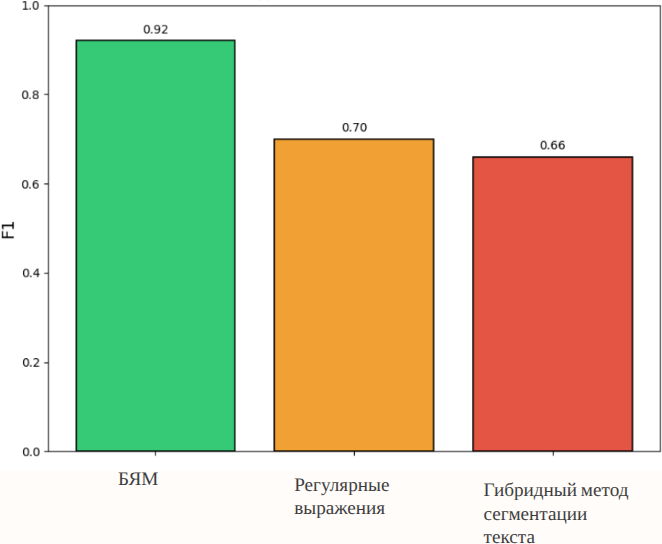
\includegraphics[width=0.9\linewidth]{images/vasexp.png}

  \caption{Эксперименты: визуализация и результаты} 
  \label{fig:vasexp}

\end{figure} 
\FloatBarrier

Эксперимент иллюстрирует, что для более точного извлечения библиографических областей требуется применение больших языковых моделей.

\section{Эксперимент на русскоязычном наборе данных}
Одной из ключевых проблем при проектировании систем интеллектуального парсинга библиографических данных является отсутствие в открытом доступе специализированных русскоязычных корпусов, размеченных в соответствии с национальными стандартами, в частности, ГОСТ. Большинство существующих наборов данных, таких как EXCITE или Grobid, ориентированы исключительно на англоязычную научно-техническую литературу и стандарты APA, MLA или Chicago. 

Для решения проблемы холодного старта и формирования репрезентативной выборки был рассмотрен массив из 7312 документов в формате  $\LaTeX$ (\texttt{*.tex}),  предоставленный специально для данной работы Математическим институтом им. В.А. Стеклова РАН. Массив документов содержит списки литературы к научным статьям, индексированным в базе данных Общероссийского математического портала Math-Net.Ru \cite{chebukov2013math}. Особенностью  данных является то, что для каждого пункта списка литературы представлены как оригинальная русская, так и переводная английская версии цитируемой публикации.

Процесс подготовки данных состоял из нескольких последовательных этапов:
\begin{enumerate}
    \item Нормализация кодировки текста: Исходные файлы поставлялись в устаревшей кодировке \texttt{CP866} (DOS Russian), использовавшейся в ранних дистрибутивах MiKTeX для совместимости с консольным выводом. Для корректной интеграции с современными токенизаторами БЯМ был разработан автоматизированный скрипт на языке Python, осуществивший пакетную транскодинговую конвертацию всего пула документов в международный стандарт \texttt{UTF-8}.
    \item Сегментация и экстракция макросов: Из структуры $\LaTeX$-документов с помощью регулярных выражений изолировалось содержимое окружения \texttt{\textbackslash begin\{thebibliography\}} \dots \texttt{\textbackslash end\{thebibliography\}}. Каждая запись, ограниченная макросами \texttt{\textbackslash Bibitem} или \texttt{\textbackslash RBibitem}, извлекалась как отдельный объект.
    \item Синтаксический разбор и конвертация: Внутренние теги издательской разметки (такие как \texttt{\textbackslash by} — авторы, \texttt{\textbackslash paper} — название статьи, \texttt{\textbackslash jour} — журнал, \texttt{\textbackslash yr} — год издания, \texttt{\textbackslash vol} — том, \texttt{\textbackslash issue} — номер, \texttt{\textbackslash pages} — страницы) парсились и агрегировались в структурированный формат \texttt{YAML}. 
    \item Генерация сырых строк по ГОСТ: На основе извлеченных атомарных полей программным путем формировалась монолитная текстовая строка («сырая» ссылка), имитирующая реальное текстовое представление пристатейного списка по ГОСТ.
\end{enumerate}

В результате выполнения описанного конвейера предобработки был сформирован итоговый профильный датасет, суммарно насчитывающий 19 430 уникальных библиографических записей, полностью готовых для проведения сравнительных экспериментов.

Целью данного этапа исследования являлось определение способности современной большой языковой модели общего назначения осуществлять синтаксический разбор без предварительного специализированного дообучения весов. 

Дизайн эксперимента строился по следующей схеме:
\begin{enumerate}
    \item Из сформированной базы данных \texttt{YAML} последовательно извлекалась сгенерированная «сырая» библиографическая строка.
    \item Строка передавалась в БЯМ в качестве входного параметра (\texttt{input}) в рамках жестко заданного системного контекста (System Prompt): \textit{«Ты — эксперт по библиографии. Извлеки данные в JSON: authors, paper, journal, year, volume, issue, pages. Если данных нет, пиши null. Отвечай ТОЛЬКО чистым JSON»}.
    \item Сгенерированный текстовый ответ модели валидировался на соответствие синтаксису JSON, десериализовался в Python-словарь и поэлементно сравнивался с эталонными полями разметки, полученными напрямую из исходных $\LaTeX$-макросов Math-Net.
\end{enumerate}

В качестве исследуемого вычислительного ядра была выбрана модель Llama-3-8B-Instruct, представленная в оптимизированном формате квантования Q4\_K\_M (4-битное квантование сбалансированного типа) в виде единого бинарного файла \texttt{.gguf}. Эксперимент разворачивался на CPU-сервере: 20 ядер, 78.5 Гб RAM под управлением инференс-движка \texttt{llama.cpp}. Использование квантованной модели 8B обусловлено необходимостью достижения приемлемой скорости генерации (в среднем 2.14 токена в секунду) в условиях отсутствия графических ускорителей (GPU).

Для математической оценки качества извлечения каждой из семи библиографических областей использовалась строгая метрика $F_1\text{-score}$, рассчитываемая на уровне отдельных токенов (Token-level) для нивелирования незначительных различий в знаках пунктуации, кавычках или служебных символах $\LaTeX$ (например, знаках неразрывного пробела \texttt{\~{}}):
\begin{equation}
Precision = \frac{|T_{true} \cap T_{pred}|}{|T_{pred}|}, \quad Recall = \frac{|T_{true} \cap T_{pred}|}{|T_{true}|}
\end{equation}
\begin{equation}
F_1 = 2 \cdot \frac{Precision \cdot Recall}{Precision + Recall}
\end{equation}
где $T_{true}$ — множество токенов в эталонном поле, а $T_{pred}$ — множество токенов в строке, извлеченной БЯМ. Общее качество модели оценивалось через интегральный показатель $Macro\ F_1$, представляющий собой среднее арифметическое оценок всех изолированных областей.

После проведения полного цикла инференса на тестовом подмножестве данных были зафиксированы показатели точности, представленные в таблице~\ref{tab:base_results}.

\begin{table}[h!]
\centering
\caption{Показатели точности извлечения данных базовой моделью Llama-3-8B-Instruct (Q4\_K\_M)}
\label{tab:base_results}
\begin{tabular}{|l|c|}
\hline
\textbf{Библиографическая область} & \textbf{Метрика Token-level $F_1$-score} \\ \hline
Авторы (\texttt{authors}) & 0,8766 \\ \hline
Название статьи/книги (\texttt{paper}) & 0,2700 \\ \hline
Журнал/Издательство (\texttt{journal}) & 0,8200 \\ \hline
Год издания (\texttt{year}) & 0,9951 \\ \hline
Том (\texttt{volume}) & 0,9613 \\ \hline
Номер выпуска (\texttt{issue}) & 0,9909 \\ \hline
Страницы (\texttt{pages}) & 0,9619 \\ \hline \hline
\textbf{Интегральный показатель Macro $F_1$} & \textbf{0,8397} \\ \hline
\end{tabular}
\end{table}


Анализ численных результатов позволяет сделать важные выводы о характере работы предобученной модели Llama-3 в задачах Zero-Shot парсинга русскоязычных академических текстов:
\begin{enumerate}
    \item Аномально низкое качество извлечения названий статей ($F_1 = 0,27$): Данный провал является центральной уязвимостью базовой модели. Его природа кроется в синтаксической специфике ГОСТ. В русскоязычной традиции название статьи графически никак не отделяется от авторов (идет сразу за ними через точку или пробел), но жестко отделяется от названия журнала двойным слэшем (\texttt{//}). Модель безошибочно определяла границу журнала, но стабильно «отрезала» значительную часть названия статьи, путая её с именами авторов, либо полностью игнорировала это поле, заполняя его значением \texttt{null}, если название содержало специфическую математическую терминологию.
    \item Высокая точность квазирегулярных сущностей: Поля «Год» ($0,9951$), «Номер» ($0,9909$) и «Страницы» ($0,9619$) распознаются моделью практически безошибочно. Это объясняется тем, что числовые паттерны, окруженные характерными маркерами (буквами «С.», «Т.», «№»), обладают сильной позиционной привязкой в механизме внутреннего внимания БЯМ, сформированной ещё на этапе предварительного обучения.
    \item Проблема языкового барьера: Поле «Авторы» ($0,8766$) продемонстрировало умеренное качество. Модель часто путалась в инициалах русских фамилий, склеенных через тильду или точку, иногда относя их к метаданным самой строки.
\end{enumerate}

Несмотря на относительно высокий интегральный показатель $Macro\ F_1 = 0,8397$, базовая архитектура Llama-3-8B-Instruct в режиме Zero-Shot непригодна для решения практических задач автоматизации библиографического контроля из-за критически низкой точности локализации названий публикаций ($F_1 = 0,27$). Модель демонстрирует глубокое непонимание специфики русскоязычных разделителей ГОСТ. Данный вывод полностью обосновывает необходимость перехода от инженерии промптов к технологиям глубокой адаптации весов модели под конкретную предметную область, что и легло в основу проведения следующего эксперимента по дообучению с использованием LoRA-адаптеров.

\section{Дообучение БЯМ с помощью LoRA-адаптера}
Для повышения качества извлечения библиографических областей из неструктурированных текстовых строк было принято решение о проведении экспериментов по контролируемому дообучению больших языковых моделей. Прямое полное дообучение всех параметров модели признано неэффективным ввиду высоких вычислительных затрат.

В связи с этим в качестве базового метода адаптации выбран алгоритм низкоранговой адаптации $LoRA$, а точнее его модификация, оптимизированная по объёму потребляемой памяти, -- $QLoRA$. $QLoRA$ внедряет небольшое число обучаемы весов, называемых адаптерами, в слои внимания замороженной базовой модели, предварительно квантованной в 4-битный форма нормализованного типа данных с плавающей запятов $NF4$.

Математическая суть модификации слоёв линейное проекции приведена в уравнении:
\begin{equation}
    W_{updated} = W_{base} + \Delta W = W_{base} + \frac{\alpha}{r} (A \cdot B)
\end{equation}
где $W_{base} \in \mathbb{R}^{d \times k}$ — замороженные веса базовой модели, $A \in \mathbb{R}^{d \times r}$ и $B \in \mathbb{R}^{r \times k}$ — матрицы низкого ранга, подлежащие обучению, $r$ — ранг адаптера ($r \ll \min(d,k)$), а $\alpha$ — коэффициент масштабирования слоев LoRA.

После чего был поставлен эксперимент на локальном CPU-сервере с 20 вычислительными ядрами процессора, 78,5 Гб оперативной памяти. В качестве среды выполнения использовалась библиотека $llama.cpp$ и её Python-обертка $llama-cpp-python$.

Однако в ходе отладки было выявлено критическое ограничение: бинарные компоненты и компилятор $llama-finetune$ на текущий момент развития экосистемы не поддерживают обратное распространение ошибки (backpropagation) через квантованные структуры тензоров (форматы типа $Q4\_K\_M$). Попытка запуска приводила к системному сбою ядра вычислений (`GGML\_ASSERT failed`). В связи с этим процесс обучения был перенесен в облачную инфраструктуру, оснащенную графическим ускорителем $NVIDIA\ Tesla\ T4$ с 16 Гб видеопамяти ($VRAM$).

Программный стек эксперимента составили:
\begin{itemize}
    \item Фреймворк высокоэффективного дообучения $Unsloth$;
    \item Библиотека управления обучением $Hugging\ Face\ TRL$ ($SFTTrainer$);
    \item Библиотека квантования $bitsandbytes$;
    \item Инструментарий визуализации $Unsloth\ Studio$.
\end{itemize}

Для проведения эксперимента из исходных файлов разметки $\LaTeX$ ($*\_utf8.tex$) подсистем библиографических списков журналов был сформирован массив данных, содержащий сырые строки и соответствующие им целевые JSON-объекты.

В ходе первой итерации автоматизированной разметки корпуса был зафиксирован систематический сдвиг левых границ извлекаемых сущностей, приведший к падению точности базовых моделей. Анализ ложноположительных срабатываний выявил ошибку избыточной предикации (\guillemotleft жадного квантификатора\guillemotright{}) в регулярных выражениях, отвечающих за первичный токенизированный парсинг. 

Применение оператора вида \texttt{.*} вместо его ленивой модификации \texttt{.*?} приводило к тому, что поисковый движок захватывал максимальную непрерывную последовательность символов. В контексте библиографии это вызывало поглощение конечных инициалов предыдущего автора началом названия статьи, либо слияние года издания с номерами страниц при совпадении синтаксических разделителей. Данный дефект разметки привел к искажению контекстных окон при обучении LoRA-адаптера, так как модель получала зашумленные векторы признаков $x_{ij}$.

Для стабилизации конвейера все жадные квантификаторы в регулярных масках были принудительно ограничены точками останова и переведены в ленивый режим работы. Повторная фильтрация корпуса исключила наложение смежных полей, что позволило повысить итоговое значение символьно-ориентированной метрики $F_1$ на этапе семантического структурирования. Сравнительный анализ структуры корректного и дефектного элементов датасета представлен в таблице~\ref{tab:dataset_error}.

\begin{table}[h!]
\centering
\caption{Анализ дефекта предобработки данных}
\label{tab:dataset_error}
\begin{tabular}{|l|p{5cm}|p{5cm}|}
\hline
\textbf{Поле JSON} & \textbf{Дефектный датасет (Итерация 1)} & \textbf{Корректный датасет (Итерация 2)} \\ \hline
\texttt{instruction} & Извлеки библиографические данные в JSON. & Извлеки библиографические данные в JSON. \\ \hline
\texttt{input} & Татаринов Я. В. Слабо неголономные системы // 1986. & Татаринов Я. В. Слабо неголономные системы // 1986. \\ \hline
\texttt{output} & Ты — эксперт по библиографии... & \{"authors": "Татаринов Я. В.", "paper": "Слабо неголономные системы", "year": "1986"\} \\ \hline
\end{tabular}
\end{table}

Именно этот скрытый дефект данных, обнаруженный в ходе пост-анализа, предопределил провал первой итерации обучения, так как модель была обучена замещать логику анализа простым циклическим копированием системного промпта.

Гиперпараметры LoRA-адаптера и процедуры обучения зафиксированы следующим образом: ранг адаптера $r = 16$, коэффициент $\alpha = 16$, целевые модули — все линейные слои ($q\_proj, k\_proj, v\_proj, o\_proj, gate\_proj, up\_proj, down\_proj$), скорость обучения $LR = 2\cdot 10^{-4}$ с линейным затуханием, оптимизатор — 8-битный $AdamW$. Базовая модель — $Llama-3-8B-Instruct$ ($bnb-4bit$). Всего было выполнено 100 шагов оптимизации с размером батча равным 2 и аккумулированием градиентов на 4 шага.

Несмотря на то, что графики функции потерь ($Loss$) в интерфейсе $Unsloth\ Studio$ демонстрировали идеальную сходимость, где замечено падение значения с 2,8 до 0,12, итоговое тестирование обученного LoRA-адаптера на контрольной выборке из 510 записей показало катастрофические результаты, усредненные по метрике $Macro\ F1$.

\begin{table}[h!]
\centering
\caption{Результаты тестирования дефектного LoRA-адаптера}
\label{tab:bad_results}
\begin{tabular}{|l|c|}
\hline
\textbf{Библиографическая область} & \textbf{Метрика Token-level F1-score} \\ \hline
Authors & 0,4039 \\ \hline
Paper & 0,3681 \\ \hline
Journal & 0,4014 \\ \hline
Year & 0,4039 \\ \hline
Volume & 0,4039 \\ \hline
Issue & 0,4039 \\ \hline
Pages & 0,4027 \\ \hline \hline
\textbf{Macro F1 Score} & \textbf{0,3983} \\ \hline
\textbf{Количество критических ошибок JSON} & \textbf{304 из 510} \\ \hline
\end{tabular}
\end{table}

Детальный анализ логов инференса (вывода) модели позволил локализовать природу аномалии. Модель не потеряла способность к генерации токенов, однако вместо формирования целевой структуры JSON, она циклически генерировала текст: \textit{«Ты — эксперт по библиографии. Извлеки данные в JSON. — — Извлеки библиографические данные в JSON...»}. 

Данное поведение обусловлено двумя факторами:
\begin{enumerate}
    \item Переобучение на мусорном паттерне (Data Poisoning): Из-за ошибки в скрипте конвертации $convert\_train2json.py$, модель выучила ложную статистическую взаимосвязь: на любую сырую строку отвечать текстом инструкции.
    \item Нарушение формата разметки токенов (Inference Prompt Mismatch): Несовпадение специальных токенов разметки начала и конца сообщений ($<|start\_header\_id|>$, $<|eot\_id|>$) во время обучения в GUI-студии и последующего скриптового тестирования привело к зацикливанию механизма внимания (Attention Loop). Модель интерпретировала управляющие токены как часть текстового ответа.
\end{enumerate}

Проведенный эксперимент наглядно иллюстрирует фундаментальный принцип инженерии данных: качество работы дообученной большой языковой модели прямо пропорционально качеству очистки и разметки входного датасета. Даже при идеальных показателях сходимости математической функции потерь на этапе обучения, дефекты структуры данных приводят к полной деградации целевой логики на этапе инференса. Данный опыт лег в основу разработки модифицированного, строго валидируемого конвейера подготовки данных, рассматриваемого в следующем разделе.

\chapter{Обсуждение результатов}

В данной главе проводится детальный анализ результатов экспериментального сравнения различных подходов к извлечению библиографии, обсуждаются качественные характеристики ошибок, оценивается вычислительная эффективность методов и описывается процесс интеграции разработанного решения в производственную среду информационной системы ИСАНД.

\section{Сравнительный анализ подходов}
На этапах локализации границ библиографических блоков и построчной сегментации записей инструмент GROBID показал наилучшие результаты при обработке англоязычного корпуса. Высокое качество парсинга обусловлено спецификой архитектуры данного инструмента: в процессе предварительного разбора PDF-файла алгоритм извлекает не только символьные цепочки, но и пространственно-геометрические параметры макета страницы. Наличие этих данных позволяет модели стабильно дифференцировать текстовые колонки, элементы колонтитулов и тело основной статьи.

Напротив, схема на базе регулярных выражений и градиентного бустинга оказалась уязвимой перед стилевым многообразием вёрстки. Детерминированные правила успешно распознают явную нумерацию вроде «<<[1]>>» или «<<[2]>>», но теряют эффективность при анализе монолитных абзацев, где ссылки разделяются обычными точками с пробелами. Сбои фиксируются и при обработке строк с выступами, если первичный программный экстрактор исказил координатную сетку PDF-слоя.

Экспериментальная проверка БЯМ на исходных текстах статей показала их слабую применимость к подзадаче $g_1$. Ограниченность контекста и размытие весов внимания на длинных цепочках токенов приводят к ошибкам детекции начала списка литературы. Наконец, из-за генеративных свойств БЯМ возникает эффект скрытого редактирования. Происходит отбрасывание строк или автокоррекция опечаток, что разрушает логику точной сегментации, где критически важен исходный синтаксис. Из этого следует, что для задач $g_1$ и $g_2$ использование детерминированных инструментов вроде GROBID остается базовым стандартом.

Картина принципиально меняется на этапе извлечения библиографических областей, где GROBID показал резкое падение качества при извлечении сложных сущностей, в то время как дообученная модель Llama-3-8B достигает высокого макро-$F_1 = 0,84$.

Низкое качество GROBID на этапе $g_3$ объясняется ограничениями CRF/BiLSTM архитектуры. GROBID решает задачу структурирования как последовательную разметку токенов в формате BIO: Begin, Inside, Outside. Условные случайные поля оперируют исключительно соседними токенами и жёсткими эвристическими признаками. Когда GROBID сталкивается с нестандартным оформлением авторов (например, инвертированный порядок «Красоткин Семён Александрович», отсутствие пробелов между инициалами «С.А.Красоткин», наличие иностранных частиц «фон», «де», «ла»), модель не может сопоставить текущий токен с глобальным смыслом записи. Точка, которая в одном стиле разделяет фамилию и инициалы, в другом стиле может завершать название журнала, что приводит к каскадной ошибке разметки и ошибочному отнесению фамилии к полю заголовка.

В свою очередь, БЯМ благодаря механизму self-attention обладают способностью улавливать глобальный семантический контекст всей записи целиком. Модель понимает, что токены, следующие сразу после начала строки и имеющие форму заглавных букв с точками, с высокой вероятностью относятся к авторам, даже если пунктуация нарушена или отсутствует. В текущей версии системы LoRA не используется, потому что эксперимент не удался из-за зашумлённых данных, а базовая модель и так даёт приемлемое качество $F_1=0,84$.

Для глубокого понимания пределов применимости разработанной системы проведён качественный анализ ошибок, классифицированный по источникам возникновения.

Наибольшее количество неустранимых ошибок связано с кумулятивным эффектом шумов на этапе извлечения текста (действие отображения $g_1$). Если библиотека PDFplumber или PyMuPDF объединяет конец одной строки с началом другой без пробела, GROBID формирует единый токен, который семантически не существует. 

Специфика библиографических данных, предоставленный из Math-Net.Ru, заключается в их синтаксической неоднородности, вызванной обилием математического аппарата в названиях публикаций. Хотя модель DeepSeek обнаружила высокую инвариантность к пунктуационным искажениям верстки, в ходе вычислительных экспериментов проявился систематический дефект. Алгоритм склонен опускать или деформировать математические выражения внутри заголовков, принудительно подменяя отсутствующие в словаре токенизатора спецсимволы на текстовые маркеры-заглушки. Данный сбой обусловлен фундаментальными особенностями авторегрессионных архитектур. Для преодоления этого барьера необходима интеграция дополнительного конвейера постпроцессинга, восстанавливающего исходные формулы с помощью регулярных масок.

Критическое значение для стабильности конвейера имеет дефект слияния независимых строк на этапе $g_2$. В единичных сценариях инструмент GROBID объединял две смежные библиографические записи, если в исходном PDF-документе отсутствовал межстрочный вертикальный интервал, а авторы отказались от сквозной нумерации списка. Передача подобного композитного токена на вход языковой модели приводила к системному сбою: Llama-3-8B пыталась агрегировать атрибуты двух разных публикаций в рамках единой JSON-схемы, что вызывало принудительное отсечение информации либо генерацию синтаксически нарушенного кода. Данный факт наглядно доказывает каскадный характер ошибок: погрешность на шаге сегментации $g_2$ полностью блокирует возможность корректного извлечения семантических полей.

Наряду с показателями полноты разбора, интеграция разработанных модулей в промышленный контур сдерживается требованиями к объёму видеопамяти и регламентированным временем отклика системы. Процедура отладки конвейера включала детальное сопоставление временных и ресурсных характеристик исследуемых подходов.

Инструмент GROBID, реализованный на языке Java и использующий компактные модели условных случайных полей, характеризуется низкими требованиями к вычислительным ресурсам и минимальным объёмом оперативной памяти. Это позволяет эффективно развертывать его в многопоточном режиме на стандартной серверной инфраструктуре общего назначения без привлечения специализированных графических ускорителей.

В свою очередь, развёртывание модели Llama-3-8B в исходной точности FP16 блокируется жёсткими лимитами видеопамяти. Проблема дефицита VRAM решена переходом к 4-битному сжатию весовых коэффициентов в формате GGUF $Q4\_K\_M$, сделав систему совместимой с доступными графическими ускорителями массового сегмента. Однако вычислительная сложность авторегрессионного декодирования накладывает ограничения на скорость обработки каждой отдельной ссылки. При анализе объёмных библиографических списков кумулятивная задержка языковой модели становится критической, что на порядок замедляет работу по сравнению с rule-based аналогами.

Архитектурный компромисс достигнут за счёт гибридизации системы, устранившей дисбаланс вычислительных скоростей. Первичная детекция и грубая сегментация возлагаются на быстродействующий детерминированный парсер, тогда как интеллектуальный семантический анализ изолированных текстовых строк выполняется большой языковой моделью в фоновом, асинхронном режиме.

\section{Внедрение в систему ИСАНД}

Разработанный конвейер интегрирован в качестве прототипа в информационную систему анализа научной деятельности (ИСАНД) в виде микросервисной архитектуры. В связи с разительным отличием в требованиях к вычислительным ресурсам, система была разделена на два независимых контура: контур первичной обработки и контур глубокого структурирования.

Интеграция разработанного модуля в информационную систему анализа научной деятельности (ИСАНД) осуществлялась по микросервисной архитектуре с использованием контейнеризации Docker.

На текущий момент в продуктивной среде ИСАНД развернут и постоянно функционирует модуль на основе GROBID. Сервис запущен в виде фонового Java-процесса, обеспечивающего REST API для приема PDF-файлов. По умолчанию все запросы направляются в grobid-worker.

Модуль на базе $Llama-3-8B-Instruct.Q4\_K\_M.gguf$ спроектирован как отдельный асинхронный Python-сервис с использованием FastAPI и библиотеки `llama-cpp-python`. На текущий момент он не развернут на общем веб-сервере ИСАНД из-за необходимости выделенного GPU-узла, но прошёл экспериментальное нагрузочное тестирование на нескольких выпусках журналов теории управления. 

Процесс взаимодействия двух модулей выглядит следующим образом:
\begin{enumerate}
    \item Пользователь загружает PDF в ИСАНД.
    \item Система отправляет файл в GROBID, получая обратно TEI/XML с сырыми записями.
    \item Сырые записи сохраняются в базу данных (обеспечивая мгновенный ответ пользователю).
    \item В фоновом режиме (через брокер сообщений) сырые строки передаются в Llama-сервис.
    \item Llama-сервис возвращает enrichment-данные (JSON с уточненными полями авторов, заголовков и т.д.), которые обновляются в базе данных ИСАНД.
\end{enumerate}
Такая двухуровневая архитектура позволяет системе не заставлять пользователя ждать 15 секунд при загрузке файла, немедленно показывая результат работы GROBID, и параллельно догружать качественную семантику с помощью БЯМ.

\section{Оценка достоверности полученных результатов}

Достоверность результатов в данной работе обеспечивается соблюдением стандартных практик машинного обучения, корректным разделением данных, обоснованным выбором метрик и фиксацией экспериментального окружения. Поскольку задача разбора библиографии чувствительна к шуму, стилевому разнообразию и артефактам препроцессинга, валидация строится на воспроизводимости условий и прозрачной оценке качества.

Обучающая, валидационная и тестовая выборки формировались на уровне целых документов, а не отдельных библиографических записей. Это исключает ситуацию, когда фрагменты одной статьи попадают в разные подвыборки, что могло бы искусственно завысить метрики за счёт контекстуального сходства. Все этапы предобработки (очистка текста, нормализация кодировок, фильтрация артефактов) применялись к каждой подвыборке независимо, без использования статистик или словарей, вычисленных по всему корпусу. Таким образом, риск утечки данных сведён к минимуму, а тестовая выборка имитирует реальные условия обработки ранее не встречавшихся публикаций.

Для оценки использовалась символьная $F_1$-мера в агрегации макро-среднего. Отказ от токеновой метрики обусловлен особенностями работы субсловных токенизаторов BPE/SentencePiece, которые по-разному сегментируют кириллические фамилии, инициалы и знаки препинания по сравнению с эталонной разметкой. Символьное сравнение напрямую отражает пригодность извлечённых полей для последующей нормализации и сопоставления с внешними базами. Макро-усреднение по полям выбрано для того, чтобы редкие, но важные элементы: соавторы, специфичные обозначения источников, DOI, -- не маскировались частотными полями вроде года издания или названия журнала.

Дообучение проводилось с использованием конфигурации LoRA-адаптеров, рекомендованной фреймворком Unsloth для моделей семейства Llama-3 ($r=16$, $\alpha=32$, \texttt{lora\_dropout}=0,05). Расширенный поиск гиперпараметров не проводился, поскольку основная цель эксперимента заключалась в проверке применимости подхода к русскоязычной библиографии, а не в поиске теоретического потолка качества. Для обеспечения воспроизводимости зафиксированы версии ключевых библиотек (\texttt{transformers}, \texttt{peft}, \texttt{unsloth}, \texttt{bitsandbytes}), параметры генерации (\texttt{temperature}=0,1, \texttt{top\_p}=0,9, \texttt{max\_new\_tokens}=512) и спецификация вычислительного окружения (CUDA 12.1, Python 3.10). Исходный код пайплайна и скрипты оценки версионированы.

Корпус Math-Net.Ru предоставлен на условиях, согласованных с правообладателем, и используется исключительно в исследовательских целях. Результаты валидны для текстовых PDF и LaTeX-исходников научных статей, где библиография оформлена отдельным разделом в конце документа. Система не оптимизирована для полностью растровых сканов низкого разрешения, постраничных сносок или документов с отсутствующим текстовым слоем, так как в этих случаях требуется отдельный этап OCR и восстановления логической структуры, выходящий за рамки текущего конвейера.

Ограниченность вычислительных ресурсов предопределила проведение одиночной итерации эксперимента без процедуры многократного усреднения по случайным инициализациям весов. Подобный подход обоснован высокой стоимостью выполнения современных больших языковых моделей, хотя полученные численные значения и остаются жестко привязанными к текущему разбиению данных. Вместе с тем, репрезентативность результатов обеспечивается за счет изоляции документов на уровне выборок, автономного препроцессинга, применения инвариантных к токенизации метрик и фиксации программно-аппаратной среды. Достигнутый уровень макро-\(F1 = 0{,}84\) на кириллическом материале доказывает состоятельность гибридной архитектуры и служит основанием для внедрения разработанного программного модуля в контур ИСАНД.

\section{Дальнейшие работы}

Факт достижения целевых метрик не исключает наличия у разработанного пайплайна архитектурных лимитов. Дальнейшая модернизация комплекса предполагает решение трех прикладных задач: оптимизация GROBID под специфику кириллических изданий, разбор распределенных по тексту библиографических сносок и внедрение фильтров для блокировки недостоверных генеративных данных.

Инструмент GROBID исторически ориентирован на англоязычный сегмент научной периодики, что приводит к падению качества на этапах $g_2$ и $g_3$ при обработке русскоязычных текстов. Это обусловлено следующими факторами: высокая вариативность антропонимов и специфические разделители.

Для решения этой задачи планируется полный цикл переобучения CRF-каскада GROBID на базе корпуса Math-Net.Ru. С помощью фреймворка \textit{grobid-trainer} PDF-файлы будут конвертированы в размеченный TEI-формат. Вектор признаков токена $x_{ij}$ будет расширен за счет кириллических словарей и регулярных выражений для детекции маркеров ГОСТ, что позволит повысить полноту извлечения до уровня англоязычных аналогов.

Текущая реализация опирается на допущение, что ссылки локализованы в едином блоке «Список литературы». Однако в гуманитарных дисциплинах доминируют постраничные сноски, также известные как footnotes. Их интеграция в конвейер требует перехода к анализу макета документа из-за следующих сложностей: сноски расположены внизу страницы и часто не отделены от основного текста жесткими маркерами; сноска может переноситься на следующую страницу. Кроме того, гуманитарные тексты активно используют сокращения: «там же», «Указ. соч.», которые бессмысленно парсить в изоляции без модуля разрешения кореферентности.

В качестве решения планируется внедрение визуально-текстовых моделей, например, класса LayoutLM или YOLO-Ref, для сегментации пространства страницы на зоны: (\textit{MainText}, \textit{Footer}, \textit{FootnoteRegion}). После извлечения зоны сноски токены будут направляться в парсер, оснащенный стековой памятью для связывания сокращенных ссылок с полными описаниями.

Использование БЯМ для написания статей привело к появлению синтаксически идеальных, но физически несуществующих библиографических записей. Поскольку структура таких «фантомных» ссылок безупречна, этапы $g_2$ и $g_3$ отработают без ошибок, и мусор попадет в базу данных. 

Для фильтрации требуется расширить математическую модель четвертым отображением верификации $g_4$, формируя композицию:
 $$ f_{\text{verified}} = g_4 \circ g_3 \circ g_2 \circ g_1
 $$ где $g_4 : C \to C \times \{0, 1\}$ — функция, сопоставляющая записи бинарный флаг истинности на основе внешних баз данных.

\begin{algorithm}[H]
\caption{Алгоритм верификации библиографической записи}
\label{alg:verify_biblio}
\begin{algorithmic}[1]
\Require Структурированный объект $c = \{\textit{authors}, \textit{title}, \textit{journal}, \textit{year}, \textit{doi}\}$
\Ensure Верифицированный объект $c_{\text{verified}}$ с флагом $V \in \{0, 1\}$

\If{$\textit{doi} \neq \emptyset$}
    \State Отправить запрос к \texttt{api.crossref.org/works/[doi]}
    \If{статус 200 \textbf{и} метаданные совпадают}
        \State \Return $(c, 1)$
    \EndIf
\EndIf

\State Сформировать поисковый запрос $S = \text{``}\textit{authors} + \textit{title} + \textit{year}\text{''}$
\State Выполнить поиск по $S$ в OpenAlex / РИНЦ
\State Вычислить косинусное сходство эмбеддингов и расстояние Левенштейна с топ-3 результатами

\If{$\text{Similarity\_Score} \ge \theta$}
    \State Обогатить $c$ валидным DOI из базы
    \State \Return $(c_{\text{enriched}}, 1)$
\Else
    \State \Return $(c, 0)$ \Comment{Потенциальная галлюцинация}
\EndIf
\end{algorithmic}
\end{algorithm}

Реализация модуля $g_4$ превратит локальный парсер в систему проверки академической добросовестности, защищающую библиометрические базы от загрязнения сгенерированным шумом.

\chapter{Заключение}

В ходе выполнения данной магистерской выпускной квалификационной работы успешно разработана и верифицирована гибридная система для авто\-ма\-ти\-зи\-ро\-ван\-но\-го разбора библиографических ссылок из научных публикаций. Актуальность иссле\-до\-ва\-ния обусловлена острой необходимостью перехода от трудоемкой ручной обработки текстов к автоматическим методам в современных сис\-те\-мах анализа научной дея\-тель\-нос\-ти (таких как ИСАНД), а также специфическими трудностями извлечения структурированных данных. К ним относятся деструктивные факторы разметки: ар\-те\-фак\-ты конвертации PDF-слоя, ошибки OCR и \guillemotleft стилевой хаос\guillemotright{} оформления источников.

Задача извлечения библиографии в работе декомпозирована на три последовательных этапа: локализация области библиографии, построчная сегментация записей и се\-ман\-ти\-чес\-кое структурирование атомарных полей. Для оценки качества на всех этапах конвейера обоснованно выбрана символьно-ориентированная метрика $F_1$. Данный подход позволяет корректно учитывать частичные перекрытия границ текстовых сущностей, возникающие из-за сдвига координат и отсутствия пробелов при парсинге PDF-документов.

Анализ результатов численных экспериментов на открытом англоязычном наборе данных и специализированном русскоязычном корпусе показал, что универсального метода, оптимального для всех этапов пайплайна, не существует. Для макро-ло\-ка\-ли\-за\-ции области библиографии наилучшие результаты продемонстрировали регулярные выражения. На этапе извлечения сырых библиографических записей наиболее эф\-фек\-тив\-ным среди рассмотренных методов оказался инструмент GROBID, достигший значения $F_1 = 0{,}97$. С задачей семантического структурирования полей из отдельных записей наилучшим образом справилась большая языковая модель Llama-3-8B без использования LoRA-ад\-ап\-те\-ров, продемонстрировав значение макро-$F_1 = 0{,}84$.

На основе полученных сравнительных характеристик спроектирована и программно реализована гибридная архитектура. В ней инструмент GROBID отвечает за сегментацию документа на отдельные записи, а модель Llama-3-8B осуществляет их финальное извлечение в структурированный формат JSON. Разработанный программный модуль успешно прототипирован в состав ИСАНД для автоматического построения кас\-то\-ми\-зи\-ро\-ван\-ных библиометрических сетей. Результаты работы прошли апробацию на профильных конференциях, а теоретические положения опубликованы в журнале \guillemotleft Системы высокой доступности\guillemotright~\cite{system_higher}.

Для дальнейших исследований остается открытым ряд научно-практических задач. Используемый на этапе сегментации инструмент GROBID ориентирован на английский язык, что требует его глубокого дообучения на русскоязычном корпусе или замены на альтернативные отечественные решения. Необходима модернизация системы для парсинга источников, заданных не в финальном списке литературы, а в постраничных и концевых сносках, характерных для гуманитарных наук. Требует решения новая фундаментальная проблема появления \guillemotleft генеративных галлюцинаций\guillemotright{} в списках литературы -- вымышленных авторами с помощью ИИ-ассистентов библиографических записей, верификация которых возможна только путем интеграции модулей внешнего семантического соответствия с API наукометрических баз Crossref и РИНЦ.

\chapter*{Благодарности}

Автор выражает благодарность Математическому институту им. В.А. Стеклова РАН за предоставленные данные.

\backmatter

\chapter{Список литературы}
\printbib

\end{document}